%%%---PREAMBLE---%%%%%%%%%%%%%%%%%%%%%%%%%%%%
\documentclass[twoside,12pt,final]{ucthesis-CA2012}
% fix for pandoc 1.14
\providecommand{\tightlist}{%
  \setlength{\itemsep}{0pt}\setlength{\parskip}{0pt}}

%--- Packages ---------------------------------------------------------
\usepackage[lofdepth,lotdepth,caption=false]{subfig}
\usepackage{fancyhdr}
\usepackage{amsmath, amssymb, graphicx}
\usepackage{xspace}
\usepackage{braket}
\usepackage{color}
\usepackage{setspace}
\usepackage{fancyvrb}
\usepackage{array}
\usepackage{ifxetex,ifluatex}
\usepackage{etoolbox}

%% for the per mil symbol
\usepackage[nointegrals]{wasysym}

%% for more attractive tables
\usepackage{booktabs}
\usepackage{longtable}
\usepackage{lscape}
\usepackage{tabularx}

\usepackage[nostamp]{draftwatermark}
% % Use the following to make modification
\SetWatermarkText{DRAFT}
\SetWatermarkLightness{0.95}

% suppress bottom page numbers on first page of each chapter
% because they overlap with text
%\patchcmd{\chapter}{plain}{empty}{}{}

%---New Definitions and Commands------------------------------------------------------

\newtheorem{theorem}{Jibberish}

\bibliography{references}

\hyphenation{mar-gin-al-ia}

% from uw_template.tex

% commands and environments needed by pandoc snippets
% extracted from the output of `pandoc -s`
%% Make R markdown code chunks work

\ifxetex
  \usepackage{fontspec,xltxtra,xunicode}
  \defaultfontfeatures{Mapping=tex-text,Scale=MatchLowercase}
\else
  \ifluatex
    \usepackage{fontspec}
    \defaultfontfeatures{Mapping=tex-text,Scale=MatchLowercase}
  \else
    \usepackage[utf8]{inputenc}
  \fi
\fi
\DefineShortVerb[commandchars=\\\{\}]{\|}
\DefineVerbatimEnvironment{Highlighting}{Verbatim}{commandchars=\\\{\}}
% Add ',fontsize=\small' for more characters per line
\newenvironment{Shaded}{}{}
\newcommand{\KeywordTok}[1]{\textcolor[rgb]{0.00,0.44,0.13}{\textbf{{#1}}}}
\newcommand{\DataTypeTok}[1]{\textcolor[rgb]{0.56,0.13,0.00}{{#1}}}
\newcommand{\DecValTok}[1]{\textcolor[rgb]{0.25,0.63,0.44}{{#1}}}
\newcommand{\BaseNTok}[1]{\textcolor[rgb]{0.25,0.63,0.44}{{#1}}}
\newcommand{\FloatTok}[1]{\textcolor[rgb]{0.25,0.63,0.44}{{#1}}}
\newcommand{\CharTok}[1]{\textcolor[rgb]{0.25,0.44,0.63}{{#1}}}
\newcommand{\StringTok}[1]{\textcolor[rgb]{0.25,0.44,0.63}{{#1}}}
\newcommand{\CommentTok}[1]{\textcolor[rgb]{0.38,0.63,0.69}{\textit{{#1}}}}
\newcommand{\OtherTok}[1]{\textcolor[rgb]{0.00,0.44,0.13}{{#1}}}
\newcommand{\AlertTok}[1]{\textcolor[rgb]{1.00,0.00,0.00}{\textbf{{#1}}}}
\newcommand{\FunctionTok}[1]{\textcolor[rgb]{0.02,0.16,0.49}{{#1}}}
\newcommand{\RegionMarkerTok}[1]{{#1}}
\newcommand{\ErrorTok}[1]{\textcolor[rgb]{1.00,0.00,0.00}{\textbf{{#1}}}}
\newcommand{\NormalTok}[1]{{#1}}
\newcommand{\OperatorTok}[1]{\textcolor[rgb]{0.00,0.44,0.13}{\textbf{{#1}}}}
\newcommand{\BuiltInTok}[1]{\textcolor[rgb]{0.00,0.44,0.13}{\textbf{{#1}}}}
\newcommand{\ControlFlowTok}[1]{\textcolor[rgb]{0.00,0.44,0.13}{\textbf{{#1}}}}

\ifxetex
  \usepackage[setpagesize=false, % page size defined by xetex
              unicode=false, % unicode breaks when used with xetex
              xetex,
              colorlinks=true,
              linkcolor=blue]{hyperref}
\else
  \usepackage[unicode=true,
              colorlinks=true,
              linkcolor=blue]{hyperref}
\fi
\hypersetup{breaklinks=true, pdfborder={0 0 0}}
\setlength{\parindent}{0pt}
\setlength{\parskip}{6pt plus 2pt minus 1pt}
\setlength{\emergencystretch}{3em}  % prevent overfull lines
\setcounter{secnumdepth}{0}

%---Set Margins ------------------------------------------------------
\setlength\oddsidemargin{0.25 in} \setlength\evensidemargin{0.25 in} \setlength\textwidth{6.25 in} \setlength\textheight{8.5 in} %8.5
\setlength\footskip{0.25 in} \setlength\topmargin{0 in} \setlength\headheight{0.25 in} \setlength\headsep{0.25 in}

%%%---DOCUMENT---%%%%%%%%%%%%%%%%%%%%%%%%%%%%
\begin{document}

%=== Preliminary Pages ============================================
\begin{ucfrontmatter}

  %%%%%%%%%%%%%%%%%%%%%%%%%%%
  % TITLE PAGE INFORMATION %
  %%%%%%%%%%%%%%%%%%%%%%%%%%%

  \title{Linking watersheds with genomics: Population genetics of the Foothill
yellow-legged Frog (\emph{Rana boylii})}

  \author{Ryan A Peek}
  \prevdegreeA{B.S. (University of California, Davis) 2002}
  \prevdegreeB{M.S. (University of San Francisco) 2010}
  \report{DISSERTATION} 
  \degree{DOCTOR OF PHILOSOPHY} 
  \degreemonth{September} \degreeyear{2018}
  %\defensemonth{September} % should be one of the following: March,
  %\defenseyear{2018}
  \chair{Michael R. Miller}  % this is your advisor
  \othermemberA{Peter B. Moyle} % This is a member of your committee
  \othermemberB{Mark W. Schwartz} % This is a member of your committee
  \othermemberC{} % This is a member of your committee (if your department requires 4 members)
  \numberofmembers{3} % should match the number of entries above (chair + othermembers)

  \field{Ecology}
  \campus{Davis}
	\maketitle
	\approvalpage
	%\copyrightpage

  %%%%%%%%%%%%%%%%%%%%%%%%%%%
  % DEDICATION PAGE INFORMATION %
  %%%%%%%%%%%%%%%%%%%%%%%%%%%
    \begin{dedication}

      \vspace*{25ex}
      \begin{center}
      \begin{Large}

        To those who love the water and listen best when their feet are wet

      \end{Large}
      \end{center}
  \end{dedication}
  \begin{acknowledgements}
    For all the curious people who have come before and hopefully after, I
    want to acknowledge you, and I hope we can do better to inspire and
    support those voices that may not have had the opportunities or
    priviledge I have had. Finishing a dissertation requires a community,
    and this dissertation would not have happened if it wasn't for the
    amazing community of family, friends, and colleagues who helped me every
    step of the way. In particular, thank you to Leslie---you are my sun and
    gravity---you held me together, anchored our family, and made it
    possible to run this crazy academic marathon. To my dearest little
    tadpoles, Connor and Genevieve, you inspire me, you make me laugh every
    day, and you remind me the world still has hope as long as we nourish
    joy and curiosity. I hope one day you forgive me for the amount of time
    I've spent staring at a computer. Thanks to my mom for all the support
    and love over the years, and thanks to my sister, who continues to
    inspire me. And for all my close friends, bandmates, and officemates
    (you know who you are), you keep me sane, you motivate me, and you
    remind me every day that I really love this crazy journey. Thank you for
    your time, humor, and general levity. And finally, thanks to my Dad, who
    has cajoled, pestered, and annoyed me for far too long to ``get a PhD''.
    . . thanks for believing it was possible even when I didn't. Also,
    please never suggest anything like this again. I also want to
    acknowledge my committee and my colleagues at the Center for Watershed
    Sciences for providing feedback, guidance, and support throughout my
    graduate student career. The Graduate Group in Ecology has been a great
    place to grow and mature as a scientist and researcher.
  \end{acknowledgements}
	%%%%%%%%%%%%%%%%%%%%%%%%%%%
  % ABSTRACT %
  %%%%%%%%%%%%%%%%%%%%%%%%%%%
  \begin{abstract}
    \addcontentsline{toc}{chapter}{Abstract}
    %todo: max 350 words

    \emph{Rana boylii} is an imperiled frog species native to CA and OR, and
    it is currently designated as a species of special concern (CDFW) in the
    state of CA. It has been petitioned as candidate for federal (USFWS) and
    state (CDFW) listing. As a lotic breeding amphibian, \emph{R. boylii} is
    tied closely to the local hydrology within the watersheds it inhabits.
    It is particularly sensitive to alterations to flow regimes. Future
    conservation of this species requires several crucial components,
    including establishing higher resolution watershed-level boundaries for
    populations across the species range, delineation of distinct population
    segments that can be utilized in conservation management, and
    quantification of relative genomic health of these groups (i.e., genomic
    diversity, measures of isolation, connectivity). We provide data on over
    700 samples across the range of the species, identify six genomically
    distinct groups, as well as subdivision at local watershed scales. These
    data are congruent with other molecular data on \emph{R. boylii},
    although we identify and add individuals from the Feather watershed as a
    distinctive group, at both population and subpopulation scales.
    Quantification and comparison of genomic variation across populations
    indicates populations in the southern coast, southern Sierra Nevada, and
    Northern Sierra/Feather basin in California should have high
    prioritization in conservation efforts due to patterns of bottlenecking
    and low genomic diversity. One major impact on \emph{R. boylii}
    populations has been river regulation, or the hydrological alteration of
    flow by dams and diversions. River regulation has been implicated as a
    cause of fundamental changes to downstream aquatic ecosystems.
    Regulation changes the natural flow regime which may restrict population
    connectivity and decrease genetic diversity in some species. Since
    population connectivity and the maintenance of genetic diversity are
    fundamental drivers of long-term persistence, understanding the extent
    that river regulation impacts these critical attributes of genetic
    health is an important goal. Foothill yellow-legged frog (FYLF;
    \emph{Rana boylii}) were historically abundant throughout many western
    rivers but have declined since the onset of regulation. However, the
    extent to which FYLF populations in regulated rivers are maintaining
    connectivity and genetic diversity is unknown. Here we use genetic
    methods to investigate the impacts of river regulation on FYLF to
    explore their potential for long-term persistence under continued
    regulation. We found FYLF in regulated rivers showed striking patterns
    of isolation and trajectories of genetic diversity loss relative to
    unregulated rivers. For example, river regulation explained the greatest
    amount of variance in population genetic differentiation compared with
    other covariates including geographic distance. Importantly, patterns of
    connectivity and genetic diversity loss were observed regardless of
    regulation level but were most prominent in locations with the greatest
    regulation intensity. Although our results do not bode well for
    long-term persistence of FYLF populations under current flow regulation
    regimes, they do highlight the power of genetic monitoring for assessing
    population health in aquatic organisms. In addition, analyses of data on
    hybridization between \emph{R. boylii} and \emph{R. sierrae} in a single
    region of the Sierra Nevada of California is shown. Cross-breeding
    between species, or hybridization in vertebrates has generally been
    considered a rare occurrence. Hybridization between species may combine
    parental genotypes in ways that yield reproductively sterile or isolated
    lineages, and hybridization events may be short-lived and difficult to
    detect. Furthermore, cross-breeding or hybridization between closely
    related taxa can promote gene flow (introgression) between species,
    which may be an important evolutionary mechanism for either
    homogenization (reversing initial divergence between species) or
    reproductive isolation (potentially leading to speciation). Here, we
    used thousands of genetic markers from nuclear DNA to detect a very rare
    hybridization event between two co-occurring frog species (\emph{R.
    boylii} and \emph{R. sierrae}) in the Sierra Nevada of California.
    Hybridization events are rare but have occurred in the Feather drainage
    between these two species, however it appears these are terminal events
    based on PCA, admixture, and tests of heterozygosity in species
    diagnostic SNPs.

    %\abstractsignature
  \end{abstract}
	\tableofcontents
\end{ucfrontmatter}
\begin{ucmainmatter}

\fancypagestyle{plain}{%
  \renewcommand{\headrulewidth}{0pt}%
  \fancyhf{}%
  \fancyfoot[C]{\thepage}
  \setlength\footskip{28pt}
}
\pagestyle{plain}

\hypertarget{reg-health}{%
\chapter{Flow regulation associated with decreased genetic health of a
river-breeding frog species}\label{reg-health}}

\hypertarget{introduction}{%
\section{Introduction}\label{introduction}}

Rivers simultaneously connect and carve the landscapes through which
they flow. Rivers provide corridors of connectivity for riparian and
aquatic organisms such as fish, amphibians, and macroinvertebrates
(Wiens 2002, Pringle 2003), while also acting as physical barriers on
the landscape for many terrestrial organisms (Voelker et al. 2013, Cazé
et al. 2016). Hydrologic connectivity (Pringle 2003) transfers energy,
organisms and ultimately genetic variation and thus is a critical
component for population persistence in dynamic systems where
populations must constantly adapt to temporal and spatial changes. In
Mediterranean climates, rivers have strong seasonal patterns associated
with cold, wet winters and warm, dry summers. Native aquatic organisms
have evolved life histories well adapted to these natural patterns,
which are both predictable and seasonal (Yarnell et al. 2010, Tonkin et
al. 2017).

River regulation, or the hydrological alteration of flow by dams and
diversions, impacts the seasonal and interannual flow variability within
a watershed. Regulation changes the natural flow regime and dramatically
alters geomorphic and hydrologic connectivity of watersheds (Poff et al.
2007), which may restrict natural population connectivity (Schick and
Lindley 2007, Shaw et al. 2016). River regulation can change flow
frequency, magnitude, duration, timing, and rate of change, which can
have significant impacts on aquatic organisms and ecological processes
(Poff et al. 2007, Yarnell et al. 2010). River regulation, and more
specifically, regulation associated with hydropower generation, has been
implicated as a cause of fundamental changes to downstream aquatic
ecosystems (Power et al. 1996, Bunn and Arthington 2002, Moyle et al.
2011). The hydrological regimes of over half of the world's largest
rivers have been altered by large dams (Nilsson et al. 2005) and only
recently has the extent of flow alteration and the associated
ecosystem-level impacts been acknowledged (Pringle 2001, Dudgeon et al.
2006, Murchie et al. 2008).

Changes to abiotic processes caused by river regulation can have a
substantial impact on biotic communities. The negative effects of river
regulation on migration and loss of spawning habitat (Fuller, Pope,
Ashton, \& Welsh, 2011; Sarah J. Kupferberg et al., 2012; Lind, Welsh,
\& Wilson, 1996; Rolls \& Bond, 2017), reductions in population
abundances and diversity (Fuller et al., 2011; Guzy, Eskew, Halstead, \&
Price, 2018; Lind et al., 1996; Sabo et al., 2017; Scribner et al.,
2016; Vörösmarty et al., 2010; Zhong \& Power, 1996), and fragmentation
(Guzy et al., 2018; Sabo et al., 2017; Scribner et al., 2016; Vörösmarty
et al., 2010; Werth, Schödl, \& Scheidegger, 2014; Zhong \& Power, 1996)
have been well documented. However, most rivers have not been regulated
for long periods (e.g., less than 100 years) compared to the time these
organisms had to adapt to pre-anthropogenic river flow. In regulated
rivers that organisms still occupy, it remains unknown whether
populations can persist long-term with continued regulation. In other
words, while some species may have persisted since regulation began in a
system (e.g., several decades), this does not necessarily mean these
populations will persist into the future under current flow regulation
regimes. Thus, exploring the potential for long-term persistence of
populations under different flow regimes is a crucial component for
guiding conservation efforts yet remains a significant gap.

One tool that can help address this gap is the integration of genetics
and hydrology to better assess the impact of river regulation on aquatic
organisms (Scribner et al., 2016). Although aquatic organisms are often
difficult to count and monitor by conventional methods, genetic
monitoring can be a powerful tool to assess population health by
revealing factors such as fragmentation and population declines. It is
widely recognized that reductions in population connectivity can
increase isolation and inbreeding, leading to a potential ``extinction
vortex'' (Gilpin \& Soule, 1986), yet there is limited understanding of
how flow alteration may impair the processes crucial for maintenance of
genetic variation and thus adaptive capacity. In addition, there is a
current pressing need for more effective and flexible watershed
management tools, particularly in relation to monitoring aquatic
populations and implementation of environmental flows (Grantham,
Merenlender, \& Resh, 2010). Thus, population genetics could be a
powerful tool to understand the influence of different flow regimes on
population health and this information could facilitate improved flow
management to better protect aquatic populations.

The river-breeding foothill yellow-legged frog (Rana boylii; FYLF)
historically occurred in lower and mid-elevation streams and rivers from
Southern Oregon to northern Baja California west of the Sierra-Cascade
crest (Stebbins, 2003). FYLF are intimately linked with river hydrology
because they have evolved to spawn in synchrony with natural flow cues
associated with seasonal spring snowmelt or rain recession periods
(Bondi, Yarnell, Lind, \& Lind, 2013; S. J. Kupferberg, 1996; S. M.
Yarnell et al., 2010; S. Yarnell, Peek, Epke, \& Lind, 2016). However,
population declines have been documented across the former range of this
species, particularly in southern California and the Sierra Nevada where
it has been extirpated from approximately 50 percent of its historical
range (Davidson, Shaffer, \& Jennings, 2002; Jennings \& Hayes, 1994).
In California, particularly in the Sierra Nevada, river regulation may
be a significant environmental stressor (Sarah J. Kupferberg et al.,
2012; Lind et al., 1996). Regulated river reaches typically alter flows
by augmenting or diverting winter and spring runoff, thereby reducing or
eliminating flow cues and disrupting natural flow regimes. Aseasonal
flow fluctuation from river regulation can scour (detach from substrate)
or desiccate FYLF egg masses, and the loss of clutches may have a
significant demographic impact because only one egg mass is laid per
year. In many regulated rivers in the Sierra Nevada, FYLF populations
are now restricted to small unregulated tributaries flowing into the
regulated mainstem.

Here, we investigate the impacts of river regulation on genetic health
of FYLF populations across three different flow regimes. Given that
population connectivity and genetic diversity are known to be play
critical roles in long-term species persistence, we explore the
association between these metrics and levels of river regulation. Our
goal is to assess the genetic health of FYLF under different river
regulation regimes to better inform the potential for long-term
persistence. Addressing this question will help to inform management and
conservation efforts for FYLF, as well as the potential utility of
genetics for future conservation monitoring efforts in aquatic species.

\hypertarget{methods}{%
\section{Methods}\label{methods}}

\hypertarget{sample-collection}{%
\subsection{Sample collection}\label{sample-collection}}

345 FYLF buccal or tissue samples were used in this study (see Table
S1). Field sampling was conducted as previously described (Heyer,
Donnelly, McDiarmid, Hayek, \& Foster, 1994), under CDFW SCP Permit
\#0006881, with IACUC protocol \#19327. Individual post-metamorphic
frogs were buccal-swabbed following established protocols (Broquet,
Berset-Braendli, Emaresi, \& Fumagalli, 2007; Goldberg, Kaplan, \&
Schwalbe, 2003; Pidancier, Miquel, \& Miaud, 2003). Each
post-metamorphic individual was comprehensively swabbed underneath
tongue and cheek for approximately one minute. Swabs were air dried for
approximately five minutes and placed in 1.5 mL microcentrifuge tubes
while in the field. Samples were stored in the laboratory at -80°C until
DNA extraction. Where possible, tail clips from tadpole larvae were
collected, and tadpoles greater than 15 mm total length were targeted
(Parris et al., 2010; Wilbur \& Semlitsch, 1990). One small
(\textless{}3mm) tail clip was taken per individual tadpole and dried on
Whatman qualitative filter paper (grade 1) and stored at room
temperature.

\hypertarget{de-novo-assembly}{%
\subsection{De novo assembly}\label{de-novo-assembly}}

To produce a high-quality genomic resource for a frog species with a
large genome size, we first interrogated a large fraction of the genome
using RAD sequencing (Baird et al., 2008; Miller et al., 2007).
Paired-end sequence data were generated from 24 FYLF individuals
(sampling details given in Table S2) across coastal and Sierra Nevada
populations from California, USA. DNA was extracted with a magnetic
bead--based protocol (Ali et al., 2016) and quantified using Quant-iT
PicoGreen dsDNA Reagent (Thermo Fisher Scientific) with an FLx800
Fluorescence Reader (BioTek Instruments). RAD libraries were constructed
using the SbfI restriction enzyme and a new RAD protocol (Ali et al.,
2016). De novo loci discovery and contig extension were carried as
previously described (Miller et al., 2012) using the alignment program
Novoalign and the genome assembler PRICE (Ruby, Bellare, \& Derisi,
2013). This pipeline resulted in a set of 77,544 RAD contigs ranging
from 300 to 800 bp (Table S3) which served as a de novo partial genome
reference for all subsequent downstream analyses.

\hypertarget{rapture-sequencing}{%
\subsection{Rapture sequencing}\label{rapture-sequencing}}

We then performed Rapture on all samples (Table S1) (2016) using 8,533
RAD capture baits (120 bp) were designed by Arbor Biosciences from the
de novo alignment (Table S4). The final Rapture library was sequenced in
50\% of an Illumina HiSeq 3000 lane. Rapture sequence data from each
individual (Table S1) were aligned against the de novo partial genome
reference using the BWA-MEM algorithm (Li, 2013; Li \& Durbin, 2010) and
saved to BAM format. SAMtools was used to sort, filter for proper pairs,
remove PCR duplicates, and index binary alignment map (BAM), as well as
merge sequences from multiple libraries (Li et al., 2009). BAM files
from the same sample were merged before indexing using SAMtools.

\hypertarget{principal-component-analysis}{%
\subsection{Principal component
analysis}\label{principal-component-analysis}}

A probabilistic framework was used to discover SNPs for PCA as it does
not require calling genotypes and is suitable for low-coverage
sequencing data (Fumagalli et al., 2013; Korneliussen, Moltke,
Albrechtsen, \& Nielsen, 2013). All Rapture analyses were conducted
using Analysis of Next Generation Sequencing Data (ANGSD) (Korneliussen,
Albrechtsen, \& Nielsen, 2014). ANGSD analyses were conducted following
methods from Prince et al (2017), with a minimum mapping quality score
(minMapQ) of 10, a minimum base quality score (minQ) of 20, and the
genotype likelihood model (GL 1) (Li, 2011). To maximize data quality,
samples with less than 100,000 aligned reads were excluded (Table S1,
S2) using and only sites represented in at least 50\% of the included
samples (minInd) were used. Settings used in ANGSD for PCA to identify
polymorphic sites included a SNP\_pval of 1e-6, inferring major and
minor alleles (doMajorMinor 1), estimating allele frequencies (doMaf 2)
(Kim et al., 2011), retaining SNPs with a minor allele frequency of at
least 0.05 (minMaf), genotype posterior probabilities were calculated
with a uniform prior (doPost 2), and the doIBS 1 and doCov 1 options
were used to generate PCA data. Principal components (PC) summarizing
population structure were derived from classic eigenvalue decomposition
and were visualized using the ggplot2 package in R (R Core Team, 2017).

\hypertarget{genetic-differentiation-and-diversity-estimates}{%
\subsection{Genetic differentiation and diversity
estimates}\label{genetic-differentiation-and-diversity-estimates}}

Mean scaled FST was used to quantify genetic differentiation between
populations (Rousset, 1997; Wright, 1943). Genome-wide FST between
population pairs was estimated by first calculating a site frequency
spectrum (SFS) for each population (doSaf) (Nielsen, Korneliussen,
Albrechtsen, Li, \& Wang, 2012) with ANGSD. The two-dimensional SFS and
global FST between each population pair were then estimated using
realSFS (Korneliussen et al., 2014). FST was calculated between each
pair of collection locations within a watershed, and the mean of all
pairwise calculations within that watershed was calculated for each
location. We calculated the river distances (distance along river
network) between locations within watersheds using the riverdist package
in R (Tyers, 2017), and used the mean pairwise river distance (km) to
all other locations within the watershed. These values were plotted and
a generalized linear model was fitted (FST \textasciitilde{} Mean River
Distance) in R (R Core Team, 2017). To calculate Watterson's θS
(Watterson, 1975), and Tajima's θ𝜋 (Tajima, 1983), we used SFS that were
estimated as described above as priors (pest) to calculate each
statistic for each site (doThetas), which were averaged to obtain a
single value for each statistic (Korneliussen et al., 2013).

\hypertarget{boosted-regression-tree-modeling-of-variance-in-fst}{%
\subsection{Boosted regression tree modeling of variance in
FST}\label{boosted-regression-tree-modeling-of-variance-in-fst}}

We used boosted regression tree (BRT) models with the R packages gbm
(Ridgeway, 2015) and dismo (Hijmans, Phillips, Leathwick, \& Elith,
2017) to assess the relative influence of river regulation as compared
to other covariates. Boosted regression trees (BRT) are suitable
frameworks for large and complex ecological datasets because they do not
assume normality, nor linear relationships between predictor and
response variables and they ignore non-informative predictor variables
(Graham et al., 2008; Steel, Peek, Lusardi, \& Yarnell, 2017). BRTs use
iterative boosting algorithms to combine simple decision trees to
improve model performance (De'ath, 2007) and provide a robust
alternative to many traditional statistical methods (Guisan et al.,
2007; Phillips, Anderson, \& Schapire, 2006). BRTs assess the relative
impact of modeled variables by calculating the number of times a
variable is selected for splitting a tree across all folds of the cross
validation. Following Steel et al.~2017, estimates of relative influence
for each predictor variable were used to evaluate the relative
contribution a variable had in predicting the response. To evaluate the
relative influence of covariates on FST, models were trained using river
distance (km), elevation (m), upstream drainage area (km2), Strahler
stream order, and number of samples per location. Stream segment data on
elevation, length, slope, stream order, and drainage area were derived
from NHD Plus attributes (U.S. Geological Survey, National Hydrography
Dataset, Digital data, accessed, August 2017 at
\url{http://nhd.usgs.gov/data.html}). In addition, Δθ (θ𝜋 − θS) was
included to assess the effect of genomic variation on FST across
regulation types.

Model training and fitting were conducted following methods previously
described in (Steel et al., 2017). To reduce overfitting, the learning
rate (also known as the shrinking rate) was set to 0.001. Stochastic
gradient boosting was utilized to reduce prediction error (De'ath, 2007)
and the fraction of training data sampled to build each tree was 0.75,
within the range as recommended by (Brown et al., 2012). Tree complexity
was set to three to allow for second and third order interaction
effects. The minimum number of observations required in the final nodes
of each tree was three. A ten-fold cross-validation technique allowed us
to determine the number of trees at which prediction error was minimized
using the cross-validation deviance. Model performance was evaluated
using the minimum estimated cross-validation deviance which maximized
the estimated deviance explained.

\clearpage

\hypertarget{results}{%
\section{Results}\label{results}}

\textbf{\emph{Rapture produces high quality genomic data for FYLF}}

To begin investigating the impact of river regulation on FYLF, we
collected frog tissue and buccal samples from 30 locations in six rivers
representing three different flow impairment levels associated with
hydropower generation. The three flow regimes assessed were: 1)
hydropeaking, where flows are pulsed on most days from late spring
through fall to provide electricity during peak-use hours and for
recreational whitewater rafting; 2) bypass, which diverts river flows
from an upstream portion of the basin to the downstream power generation
facilities; and 3) unregulated, a largely natural flow regime where no
upstream controls exist to regulate flows (Figure 1). Flow data were
obtained for each river reach using proximal USGS gaging stations (Table
S5). We sampled a total of 345 FYLF from sites in three major watersheds
(Yuba, Bear, and American) in the northern Sierra Nevada of California
(Figure 1A; Table 1). The six study rivers share a similar Mediterranean
climate, underlying geology, watershed aspect (west-slope), stream
morphology (riffle-pool), and vegetative communities, but differ in the
intensity of flow regulation (Steel et al., 2017). Although river
regulation occurs in all three of the study watersheds, both the North
Yuba and North Fork (NF) American are unregulated whereas the Middle
Fork (MF) American is the only river that has a hydropeaking flow regime
(Figure 1A).

To generate genetic data from the samples, we performed RAD Capture
(a.k.a. Rapture) (Ali et al., 2016) on the samples by generating SbfI
RAD libraries, capturing a subset of the RAD loci using 8,533 baits (see
Methods), and sequencing the resulting library on an Illumina HiSeq. We
then aligned the sequencing reads from each sample to a de novo RAD
assembly (see Methods). The mean number of filtered alignments across
all 345 samples was 324,928. For downstream analysis, we selected
individuals that had greater than 100,000 alignments (n=277), which
provided sufficient data to investigate population genetic attributes at
broad and fine geographic scales (see below). FYLF are cryptic, and
often occur in low densities within the study area. Thus, we retained a
minimum of three individuals per site, and the mean number of samples
per site was approximately nine (Table 1). With genomic data, population
genetic parameters can be accurately estimated from even low sample
numbers (Hotaling et al., 2018), and genomic analyses in non-model
organism often use fewer loci (Narum, Buerkle, Davey, Miller, \&
Hohenlohe, 2013). We conclude that the sequence data we obtained should
be appropriate for population genetic analyses across our study area.

\textbf{\emph{Anomalous genetic pattern in highly regulated reach of
Middle Fork American watershed}}

To assess FYLF population structure across the collection locations, we
used ANGSD (Korneliussen et al., 2014) to discover 44,406 SNPs and
perform principal component analysis (PCA; see Methods), which provides
a dimensionless comparison of all samples. The first two principal
components revealed four main groups corresponding to the Yuba, Bear,
North Fork (NF) American, and Middle Fork (MF) American samples (Figure
2A). Unlike the Yuba watershed where all rivers clustered as one group,
the two rivers within the American watershed (the NF American and MF
American) were separated by both PC1 and PC2. Although the NF American
watershed clustered closely with the adjacent Bear watershed, the MF
American showed a surprisingly high degree of genetic differentiation
from other locations (Figure 2A). These data suggest that there is less
genetic differentiation between the NF American and the Bear watersheds,
than between the NF and MF American watersheds. We conclude that
measurements of overall genetic differentiation in FYLF from our study
area largely conform to watershed and geographic expectations, with the
exception of the American watershed, which shows a surprisingly high
degree of genetic differentiation between the North (unregulated) and
Middle (hydropeaking) Forks.

To further investigate patterns of genetic variation within the American
Watershed, we performed two PCAs, one on samples from the NF American,
and the other on samples from the MF American. The PCA of the NF
American showed minimal differentiation among locations, with different
study sites blending together and weak patterns of population structure
(Figure 2B). In contrast, PCA of the MF American showed strong
differentiation between sites (Figures 2C, 2D). The MF American PCA
completely resolved all sites, with the first component (PC1) strongly
differentiating the samples in the hydropeaking reach from all other
sites in the MF American. This pattern may be due to the differential
river regulation between the two rivers; the NF American is unregulated
and has weak PCA differentiation, whereas the MF American has a higher
level of river regulation and all sites form distinct genetic clusters,
indicative of reduced gene flow among sites within the MF American.
River regulation is the strongest predictor of genetic isolation with
FYLF in the Northern Sierra

To assess how patterns of genetic differentiation are associated with
river regulation across our entire study area, we estimated pairwise FST
(Wright, 1943) between all collection locations within a river for all
six rivers. We then plotted the scaled mean pairwise FST {[}mean FST /
(1-mean FST){]} (Rousset, 1997) for each location against the mean river
distance (the average distance along the river network from each
collection location to every other location within that study river).
Furthermore, each location was categorized by regulation level of
closest mainstem location (see Methods). While there was a clear
relationship between FST and river distance (as shown by the slope of
regression lines in Figure 3A), there was a striking pattern of elevated
FST by regulation type (Figure 3A). Even the bypass regulation type
showed a distinct pattern of elevated FST. For instance, regulated
rivers with locations separated by less than 10km had FST values
comparable to unregulated locations separated by mean river distances
over 30 km. Hydropeaking was the most extreme pattern of the three
regulation types and showed highly elevated FST values with the steepest
regression coefficient. The baseline FST or global mean increased by
over 0.1 between the unregulated (mean FST=0.141), and regulated
locations (global mean for bypass FST=0.256, hydropeaking FST=0.278).
This suggests a greater degree of isolation within sites in regulated
river reaches compared with FYLF populations in unregulated reaches as
larger FST values represent reductions in heterozygosity due to
population subdivision (Slatkin, 1987). We conclude FYLF in regulated
rivers show patterns of greater population isolation and loss of
heterozygosity compared to frogs in unregulated locations.

To investigate the relative influence of river regulation compared to
other covariates such as river distance on genetic differentiation
(i.e.~FST), we used boosted regression tree (BRT) modeling. Covariates
included flow regime alteration type, river distance, watershed
variables derived from National hydrology data (NHD), topographic data,
and allele frequency spectrum skew (see below, Methods). We found flow
regulation explained the greatest amount of variance in FST (Figure 3B).
Thus, river regulation has a larger relative influence than mean river
distance between sampling locations, which is often the most important
factor influencing genetic differentiation (Rousset, 1997; Slatkin,
1987; Wright, 1943). We conclude there is a pattern of isolation and
limited connectivity between populations in regulated reaches.

\textbf{\emph{River regulation strongly correlated with decreasing
genetic diversity in FYLF}} To investigate the association between river
regulation and genetic diversity trajectory (stable, increasing, or
decreasing), we summarized patterns of genetic variation using two
estimators of θ (4Nμ): Tajima's θ (θ𝜋) is based on the average number of
pairwise differences (Tajima, 1983), and Watterson's θ (θS) is based on
the number of segregating sites (Watterson, 1975) (see methods). These
estimators are influenced by the demographic history of a population and
provide information on the trajectory of changes in genetic diversity.
When genetic diversity has been stable, these estimates should be equal;
when genetic diversity has been increasing, θ𝜋 \textgreater{} θS; and
when genetic diversity has been decreasing, θS \textgreater{} θ𝜋. We
found zero populations sampled within regulated watersheds had evidence
of increasing genetic diversity (e.g., a θ𝜋 − θS that was less than
zero) (Figure 4A). The regulated locations showed a clear trajectory of
genetic diversity loss (Figure 4A, 4B). Three of the four hydropeaking
locations had the highest values of Δθ (θ𝜋 − θS), and the global mean
was significantly different from other regulation types. Although some
tributary populations within unregulated watersheds also showed signs of
genetic diversity loss, the mean genetic diversity trajectory at
unregulated locations was largely neutral (Figure 4B). This indicates
populations in the northern Sierra Nevada which are already limited in
number are losing genetic variation, and river regulation appears to be
exacerbating these patterns. We conclude there is evidence of recent
genetic diversity loss across populations in the regulated river
systems, regardless of regulation type.

\hypertarget{discussion}{%
\section{Discussion}\label{discussion}}

Although massive parallel sequencing (MPS) technologies have the
potential to facilitate collection of high-quality genetic data in
virtually any species, a number of challenges still remain for many
species including low quality or non-existent reference genomes,
large/complex/repetitive genomes, and high cost of processing/sequencing
in studies with many samples. Amphibians are particularly challenging as
many species have very large genome sizes (Nunziata, Lance, Scott,
Lemmon, \& Weisrock, 2017) for example, there are only two frog
reference genome assemblies available as of 2018 (Hellsten et al., 2010;
Sun et al., 2015). Our results demonstrate that Rapture (Ali et al.,
2016) is a suitable method to rapidly and inexpensively discover a large
number of loci in a frog species with a complex genome. In this study,
we used new RAD sequencing and RAD capture (Rapture) methods (Ali et
al., 2016) to generate high-quality genomic data suitable for
discovering and genotyping many single nucleotide polymorphisms (SNPs)
in FYLF. Based on this dataset, we were able to successfully
characterize patterns of genetic variation within FYLF as well as design
a set of RAD capture baits that can be used as a genetic monitoring
resource for FYLF (and likely other ranid species). This highlights that
the collection of genetic information, even from large numbers of
samples or in complex genomes, is no longer a limitation with current
genomic methods such as RAD and Rapture.

Demographic connectivity is widely recognized as a fundamental driver of
long-term population persistence (Fahrig \& Merriam, 1985; Taylor,
Fahrig, Henein, \& Merriam, 1993). Populations must adapt over time and
connectivity is a major way to transfer genetic information. For
example, previous studies have shown that adaptation can occur by
spreading specific alleles across large geographic distances (Miller et
al., 2012; Prince et al., 2017). In many regulated river reaches in the
Sierra Nevada, FYLF now occur in isolated locations, breeding in
tributaries rather than mainstem habitats. However, since these frogs
have the potential to move long distances (FYLF have been observed
moving over 1 km per day (Bourque, 2008)), the extent to which current
population connectivity has been lost due to river regulation remains
unknown. Examining pairwise FST, revealed a major decrease in
connectivity in populations in regulated systems, even with limited
river regulation (i.e., bypass reaches). Usually isolation by distance
patterns best describe variation in genetic data, yet the primary factor
influencing genetic differentiation among these rivers is hydrologic
alteration (Figure 3B). Thus, despite being able to move long distances,
FYLF have not been able to maintain population connectivity in regulated
rivers. This demonstrates that even in species that can move relatively
long distances and pass potential physical barriers (e.g.,
infrastructure such as dams, canals, and reservoirs likely do not
represent barriers to movement of FYLF) loss of connectivity may still
occur and can be revealed with genetic analysis.

Genetic diversity is also a critical component for long-term population
persistence because it is closely related to the evolutionary capacity
for adaptation to environmental changes (Frankham, 2002; Hoffmann \&
Sgrò, 2011; Ishiyama, Koizumi, Yuta, \& Nakamura, 2015; Lande \&
Shannon, 1996). In some cases, isolated populations can maintain genetic
diversity when they are sufficiently sized (Whiteley et al., 2010),
however, species of conservation concern typically have small and/or
declining populations and thus may be susceptible to genetic diversity
loss (Frankham, 2002; Krohn et al., 2018). Throughout the Sierra Nevada,
FYLF have largely disappeared from regulated mainstem rivers, but the
extent to which existing populations have been able to maintain genetic
diversity is unclear. Strikingly, our analysis revealed that every
single population within the regulated watersheds exhibits a trajectory
of genetic diversity loss. Thus, genomic analysis of molecular variation
provides a powerful lens to discover and assess trajectories of genetic
diversity.

Our analyses, using metrics that serve as a reasonable proxy for genetic
health, does not bode well for the long-term persistence of FYLF
populations in regulated rivers in the Sierra Nevada. Many of these FYLF
populations are already losing genetic diversity and given their small
size and reduced connectivity the effects of inbreeding will likely
exacerbate their problems. FYLF have evolved in river systems with
consistent hydrologic seasonality and predictability, despite
inter-annual variation. Flow regulation has altered patterns of
hydrologic seasonality and predictability in many watersheds (Sarah J.
Kupferberg et al., 2012). Long-term population persistence may still be
possible if conservation efforts utilize methods that promote or
maintain genetic health and increase population connectivity. For
example, simulations by Botero et al. (2015) demonstrated adaptation
persisted in modeled populations through large environmental
changes---if phenotypic strategies were appropriate before and after the
change---but modeled populations declined rapidly when the current
strategy was a mismatch to the current environment. Thus, FYLF
conservation efforts should focus on river reaches where flow management
may provide opportunities to more closely mimic local natural flow
regimes and thus improve hydrologic connectivity.

Detecting evolutionary responses to within- and among-year changes in an
ecological or hydrological context has previously been difficult.
However, utilizing genetic data can fill these gaps and provide a highly
informative process for identifying the impacts of anthropogenic and
environmental change on the process of adaptation (Botero et al., 2015;
Kahilainen, Puurtinen, \& Kotiaho, 2014). We demonstrate that an aquatic
species that has adapted to local hydrology patterns shows poor genetic
health (i.e., clear patterns of decreased connectivity and trajectories
of genetic diversity loss). Our results highlight the potential impact
of river regulation on aquatic organisms and their potential for long
term persistence. In the future, similar genetic approaches could be
used in many other contexts to explore the impacts of river regulation
on aquatic organisms. Taken together, our results demonstrate that
genetic monitoring can be a powerful tool for assessment of population
health and should be a critical component of conservation management in
aquatic organisms.

\textbf{Data Archiving Statement:} Should the manuscript be accepted,
the data supporting the results will be archived in an appropriate
public repository such as Dryad, and the data DOI will be appended to
the end of the article.

\texttt{\{r\ maxdelays,\ results="asis",\ echo=Fevalrary(knitr)\ kable(max\_delays,\ \ \ \ \ \ \ \ col.names\ =\ c("Airline",\ "Max\ Arrival\ Delay"),\ \ \ \ \ \ \ caption\ =\ "Maximum\ Delays\ by\ Airline",\ \ \ \ \ \ \ caption.short\ =\ "Max\ Delays\ by\ Airline",\ \ \ \ \ \ \ longtable\ =\ TRUE,\ \ \ \ \ \ \ booktabs\ =\ TRUE)}

The last two options make the table a little easier-to-read.

\hypertarget{hybrids}{%
\chapter{Hybridization between two sympatric ranid frog species in the
northern Sierra Nevada, California}\label{hybrids}}

\hypertarget{introduction-1}{%
\section{Introduction}\label{introduction-1}}

Landscape changes can influence species demography and migration
patterns (Li et al. 2017) which can change rates of gene flow within
species. Changing migration rates and population sizes can influence
population structure; thus, over time, landscape changes can cause
significant changes in genetic diversity within a species. Furthermore,
cross-breeding or hybridization between closely related taxa can promote
gene flow (introgression) between species, which may be an important
evolutionary mechanism for either homogenization (reversing initial
divergence between species), speciation (from reproductive isolation of
hybrid populations), or adaptation (transfer of adaptive alleles)
(Mallet 2007, Abbott et al. 2013, Barrera-Guzmán et al. 2018).

Hybridization events in vertebrates may be rare, or rarely detected, and
thus identifying potential hybridization can be difficult and may be
affected by sampling design, timing, and resolution of genetic markers.
Therefore, occurrences of hybridization likely remain unknown,
particularly in cryptic taxa. Assessing population admixture or
detecting potential hybridization has previously been challenging;
however, modern genetic methods provide a powerful approach to assess
populations at fine geographic and evolutionary scales (Ali et al. 2016,
Prince et al. 2017).

We investigate the potential for hybridization in two sympatrically
occurring endemic frog species in the Sierra Nevada of California.
Foothill yellow-legged frogs, \emph{Rana boylii}, (Baird 1856)
historically occurred in lower and mid-elevation (\textless{}1500 m)
streams and rivers from Southern Oregon to northern Baja California west
of the Sierra-Cascade crest (Stebbins 2003), whereas Sierra Nevada
yellow-legged frogs, \emph{Rana sierrae}, (Camp 1917) typically occurred
from 1500 m to over 3600 m in lakes and streams (Stebbins 2003,
@zweifel\_ecology\_1955). Population declines have been documented
across the former range of both of these species; \emph{R. sierrae} has
been extirpated from over 90 percent of its historical range (Drost and
Fellers 1996) (Vredenburg 2004) while \emph{R. boylii} has been
extirpated from 50 percent of its historical range (Jennings and Hayes
1994, Davidson et al.~2002). Both species are of conservation concern;
in 2014, the U. S. Fish and Wildlife Service (USFWS) listed \emph{R.
sierrae} as endangered under the U. S. Endangered Species Act (ESA)
(USFWS 2014), and \emph{R. boylii} is listed as a species of special
concern in California and is a candidate for listing under the
California and federal ESAs.

Unlike other ranid frog species with broad areas of potential
intergradation (Shaffer et al. 2004), \emph{R. boylii} and \emph{R.
sierrae} only rarely occur sympatrically. Zweifel (1955) described one
historical location where these two species co-occurred, in Butte County
near DeSabla. Currently the only known location where both species are
found is several tributaries to the Feather River in the northern Sierra
Nevada, California (Figure 1). Hybridization between these species has
not previously been documented. Furthermore, breeding experiments by
Zweifel (1955) between \emph{R. sierrae} (formerly known as \emph{R.
muscosa}) and \emph{R. boylii} yielded very low viability in
fertilization and high incidences of embryological
abnormalities---indicating a post-zygotic barrier between the species.
However, these experiments only crossed female \emph{R. sierrae} with
male \emph{R. boylii}, and the individuals were from very different
California regions (e.g., Butte and Nevada County vs.~Contra Costa
County). \emph{Rana boylii} and \emph{R. sierrae} species have very
similar morphology and habitat preferences in areas where they co-occur;
thus assigning individuals to species is difficult and imprecise using
field identification methods. This presents a challenge for management
because these sympatric species have different conservation status and
management objectives. We employed modern genetic methodology to better
understand \emph{R. sierrae} and \emph{R. boylii} where their ranges
overlap. We investigated three primary questions:
\begin{enumerate}
\def\labelenumi{\arabic{enumi}.}
\tightlist
\item
  Can hybridization be detected between two sympatrically occurring
  threatened and endangered (ESA) frog species in the Sierra Nevada
  using data generated from genome-wide single nucleotide polymorphisms
  (SNPs);
\item
  If hybrids can be detected, do genetic signatures suggest hybrid
  viability (i.e., can hybrids reproduce, leading to introgression
  between species);
\item
  Using coalescent modeling, are migration rates between species in
  sympatrically occurring populations higher than in allopatrically
  occurring populations in adjacent watersheds?
\end{enumerate}
\hypertarget{materials-and-methods}{%
\section{Materials and Methods}\label{materials-and-methods}}

\hypertarget{sampling-and-dna-extraction}{%
\subsection{Sampling and DNA
Extraction}\label{sampling-and-dna-extraction}}

To investigate potential hybridization between \emph{R. sierrae} and
\emph{R. boylii}, a total of 458 tadpole tail clips, buccal swabs, or
tissue samples were compiled. Samples were identified to species in the
field as either \emph{R. boylii}, \emph{R. sierrae}, or ``unknown'',
which were individuals which could not be visually confirmed as either
species (Stebbins 2003). The samples were collected between 1992 and
2016, from three watersheds in the Sierra Nevada (the Feather, Yuba, and
American) (Table S1). All unknown individuals were from Feather
watershed localities.
\begin{landscape}
\begin{longtable}[t]{l|l|r|l|l|l|l}
\caption{\label{tab:tableS1}Sample Sites}\\
\hline
Locality & River & No. Samples & Lat. & Lon. & Elev (m) & Watershed (HUC8)\\
\hline
\endfirsthead
\caption[]{\label{tab:tableS1}Sample Sites \textit{(continued)}}\\
\hline
Locality & River & No. Samples & Lat. & Lon. & Elev (m) & Watershed (HUC8)\\
\hline
\endhead
MFA-AMEC & MFA & 5 & 38.934 & -120.9436 & 240 & American\\
\hline
MFA-GASC & MFA & 1 & 38.9665 & -120.9325 & 242 & American\\
\hline
MFA-TODC & MFA & 6 & 38.9638 & -120.9216 & 368 & American\\
\hline
MFA-US-R & MFA & 1 & 39.0075 & -120.7316 & 360 & American\\
\hline
NFA & NFA & 12 & 39.1079 & -120.9227 & 363 & American\\
\hline
NFA-BUNC & NFA & 8 & 39.0376 & -120.9103 & 286 & American\\
\hline
NFA-EUCHDS & NFA & 3 & 39.1849 & -120.762 & 580 & American\\
\hline
NFA-INDC & NFA & 3 & 39.0567 & -120.9085 & 296 & American\\
\hline
NFA-LyonsPk & NFA & 11 & 39.2067 & -120.3113 & 2529 & American\\
\hline
NFA-POND & NFA & 2 & 38.9999 & -120.9406 & 241 & American\\
\hline
NFA-ROBR & NFA & 6 & 39.1045 & -120.9267 & 400 & American\\
\hline
NFA-SHIC & NFA & 8 & 39.0417 & -120.9009 & 341 & American\\
\hline
NFA-SLAR & NFA & 5 & 39.0987 & -120.9255 & 356 & American\\
\hline
NFMFA-SC & NFMFA & 7 & 39.0224 & -120.7369 & 522 & American\\
\hline
RUB-HighlandDS & RUB & 18 & 38.9615 & -120.2422 & 2312 & American\\
\hline
RUB-HighlandLk & RUB & 29 & 38.9573 & -120.2418 & 2383 & American\\
\hline
RUB-LC-US & RUB & 1 & 38.9889 & -120.69 & 415 & American\\
\hline
RUB-USPH & RUB & 5 & 38.9993 & -120.7233 & 361 & American\\
\hline
RUB-Zitella & RUB & 9 & 38.9595 & -120.227 & 2335 & American\\
\hline
RUB-ZitellaLk & RUB & 2 & 38.9604 & -120.2316 & 2337 & American\\
\hline
SFA-CAMI & SFA & 2 & 38.8115 & -120.5787 & 725 & American\\
\hline
FEA-BeanCk & FEA & 60 & 39.9774 & -121.091 & 1397 & Feather\\
\hline
FEA-EBNFF & FEA & 6 & Unknown & Unknown & Unknown & Feather\\
\hline
FEA-GoldLk & FEA & 4 & 39.9416 & -121.136 & 1816 & Feather\\
\hline
FEA-LoneRockCk & FEA & 3 & 40.2012 & -120.6453 & 1563 & Feather\\
\hline
FEA-MillCk & FEA & 4 & 39.9591 & -121.1573 & 1891 & Feather\\
\hline
FEA-RockLkBucksCk & FEA & 1 & 39.9403 & -121.1499 & 2102 & Feather\\
\hline
FEA-RockLkSilver & FEA & 8 & 39.9409 & -121.1422 & 1902 & Feather\\
\hline
FEA-SFRockCk & FEA & 27 & 39.8789 & -121.0022 & 1470 & Feather\\
\hline
FEA-SPANISH-BGulch & FEA & 5 & 39.9546 & -121.089 & 1283 & Feather\\
\hline
FEA-SPANISH-RockCk & FEA & 1 & 39.9445 & -121.0221 & 1090 & Feather\\
\hline
FEA-SPANISH-SilverCk & FEA & 3 & 39.9377 & -121.0849 & 1189 & Feather\\
\hline
FEA-SPANISH-Wapaunsie & FEA & 1 & 39.9523 & -121.0373 & 1096 & Feather\\
\hline
FEA-SpanishCk & FEA & 26 & 39.9541 & -121.0541 & 1192 & Feather\\
\hline
NFF-Poe & NFF & 1 & 39.736 & -121.4702 & 284 & Feather\\
\hline
FORD-Mossy-P1 & FORD & 1 & 39.381 & -120.4623 & 2157 & Yuba\\
\hline
FORD-Mossy-P2 & FORD & 3 & 39.3852 & -120.4714 & 1998 & Yuba\\
\hline
FORD-Mossy-P3 & FORD & 2 & 39.3765 & -120.4603 & 2158 & Yuba\\
\hline
FORD-MossyDS & FORD & 19 & 39.3853 & -120.4728 & 1984 & Yuba\\
\hline
FORD-MossyPond & FORD & 34 & 39.3781 & -120.4701 & 2106 & Yuba\\
\hline
FORD-NorthCkTrib & FORD & 34 & 39.3869 & -120.451 & 2090 & Yuba\\
\hline
MFY-OREGCk & MFY & 10 & 39.4419 & -121.0575 & 620 & Yuba\\
\hline
MFY-Remmington & MFY & 1 & 39.4137 & -120.9912 & 620 & Yuba\\
\hline
MFY-US-OH & MFY & 7 & 39.413 & -120.9903 & 624 & Yuba\\
\hline
NFY & NFY & 12 & 39.5119 & -120.9774 & 705 & Yuba\\
\hline
NFY-SLATE-CGRav & NFY & 3 & 39.6928 & -120.9258 & 1457 & Yuba\\
\hline
NFY-SLATE-Onion & NFY & 3 & 39.6355 & -121.0395 & 1300 & Yuba\\
\hline
SFY & SFY & 1 & 39.3539 & -120.7342 & 890 & Yuba\\
\hline
SFY-FallCk & SFY & 5 & 39.3553 & -120.7371 & 884 & Yuba\\
\hline
SFY-HUMBUG & SFY & 1 & 39.3637 & -120.921 & 877 & Yuba\\
\hline
SFY-LOGA & SFY & 3 & 39.3691 & -120.8526 & 1201 & Yuba\\
\hline
SFY-MCKI & SFY & 3 & 39.368 & -120.8354 & 1084 & Yuba\\
\hline
SFY-MISC & SFY & 7 & 39.361 & -120.8814 & 1095 & Yuba\\
\hline
SFY-RockCk & SFY & 3 & 39.3298 & -120.9863 & 594 & Yuba\\
\hline
SFY-Scotchman & SFY & 3 & 39.3293 & -120.777 & 1167 & Yuba\\
\hline
SFY-ShadyCk & SFY & 9 & 39.3543 & -121.059 & 675 & Yuba\\
\hline
\end{longtable}
\end{landscape}
The Yuba and American watersheds share a similar Mediterranean climate,
underlying geology, watershed aspect (west-slope), and vegetative
communities. The Feather watershed shares a similar climate but has a
slightly different underlying geology and aspect than that of other
watersheds in the Sierra Nevada. The Feather watershed lies in the
transition zone of the northern Sierra Nevada and the Cascades/Basin and
Range Province, and thus the landscape in the northern portion of the
watershed is comprised largely of volcanic bedrock while the southern
portion is largely granitic (Durrell 1988). Field sampling was conducted
following methods in Heyer et al. (1994) under CDFW SCP Permit \#0006881
and Federal permit TE-40087B-0 with IACUC protocol \#19327 and
\#04718-001. Individual post-metamorphic frogs were buccal-swabbed
following established protocols (Goldberg et al.~2003, Pidancier et
al.~2003, Broquet et al.~2007). Each post-metamorphic individual was
comprehensively swabbed underneath tongue and inside of both cheeks for
approximately 30 sec to one minute. Swabs were air dried for
approximately five minutes and placed in 1.5 mL microcentrifuge tubes
while in the field or placed in lysis buffer (Goldberg et al.~2003).
Dried samples were stored in the laboratory at -80°C until DNA
extraction. Where possible, tail clips from tadpole larvae were
collected, and tadpoles greater than 15 mm total length were
targeted(Wilbur and Semlitsch 1990, Parris et al.~2010). One clip was
taken per individual tadpole and dried on Whatman filter paper (grade 1)
and stored at room temperature or in 95\% ethanol. DNA was extracted
from ethanol-stored samples using Qiagen DNeasy kits following
manufacturer protocol and stored at -20°C. DNA was extracted from dried
buccal swabs and tail clips using an Ampure magnetic bead-based protocol
(Ali et al.~2016) and stored at -20°C.

\hypertarget{rapture-sequencing-1}{%
\subsection{Rapture Sequencing}\label{rapture-sequencing-1}}

To produce a high-quality genomic resource for frog species with large
genome sizes, we interrogated a significant fraction of the \emph{R.
boylii} genome using RAD sequencing with SbfI (Miller et al.~2007, Baird
et al.~2008, Ali et al.~2016). Paired-end sequence data were generated
using 24 \emph{R. boylii} individuals (Table S2). RAD libraries were
constructed following the protocol described in (Ali et al.~2016). De
novo locus discovery and contig extension were carried out as previously
described (Miller et al.~2012) using the alignment program Novoalign and
the genome assembler PRICE (Ruby et al.~2013). This resulted in a set of
77,544 RAD contigs ranging from 300 to 800 bp which served as a de novo
partial genome reference for all subsequent downstream analyses (File
S3: de novo). We next removed loci with five or more SNPs, and randomly
selected 10,000 loci from the remaining subset. Of these 10,000 loci,
8,533 were successfully designed into 120 bp RAD capture baits by Arbor
Biosciences (File S4: Baits). Sample libraries were prepared for
sequencing following RAD Capture (Rapture) methods outlined in Ali et
al. (2016). These samples were then then used to identify putative
high-quality SNPs following sequencing.

Sampled individuals were aligned against the de novo partial genome
reference using the BWA-MEM algorithm (Li and Durbin 2010, Li 2013), and
converted to BAM format and filtered for properly paired alignments
using Samtools (File S1). Next, alignments from three different
sequencing runs on an Illumina HiSeq were merged together and duplicates
were removed using Samtools (Li et al.~2009). For all downstream
analysis, we selected individuals that had greater than 25,000
alignments (n=311), which provided sufficient data to investigate
population genetic attributes at broad and fine geographic scales (Table
S5). To generate SNP (i.e., segregating site) data, a probabilistic
framework was used for all population genetic analyses as it does not
require calling genotypes and is suitable for low-coverage sequencing
data (Korneliussen et al.~2013, Fumagalli et al.~2013). SNP discovery,
minor allele frequencies (MAF) estimates, and genotype probabilities
were conducted using ANGSD (Korneliussen et al.~2014). ANGSD analyses
were conducted following methods from Prince et al. (2017), with a
minimum mapping quality score (minMapQ) of 10, a minimum base quality
score (minQ) of 20, the genotype likelihood model (GL 1), specifying the
RAPTURE bait locations using the -sites flag, and only sites represented
in at least 50\% of the included samples (minInd) were used.
Furthermore, genomic sites were designated as polymorphic only if MAFs
were greater than 0.05 and the probability of the site not being
polymorphic was less than 1e-6. Using this approach, over 44,000
polymorphic sites were identified across all \emph{R. boylii} study
samples.

\hypertarget{pca-admixture}{%
\subsection{PCA \& Admixture}\label{pca-admixture}}

To assess population structure and coancestry, ANGSD was used to
generate PCA and NGSadmix was used to calculate admixture. Settings used
in ANGSD for PCA to identify polymorphic sites included a SNP\_pval of
1e-6, inferring major and minor alleles (doMajorMinor 1), estimating
genotypic likelihoods (GL 1), estimating allele frequencies (doMaf 2)
(Kim et al.~2011), retaining SNPs with a minor allele frequency of at
least 0.05 (minMaf), specifying the RAPTURE bait locations using the
-sites flag, estimation of genotype posterior probabilities using a
uniform prior (doPost 2), and the -doIBS 1 and -doCov 1 options.
Principal components (PC) summarizing population structure were derived
from classic eigenvalue decomposition and were visualized using the
ggplot2 package in R (R Core Team 2017). To assess admixture between
\emph{R. sierrae} and \emph{R. boylii}, genotype likelihood data (-GL 2)
was generated in ANGSD with the same settings as above, in addition to
retaining only SNPs that were shared in at least of 50\% of the samples,
-doPost 2, -doGLF 2, and limiting to higher quality alignment data
(-minMapQ 10, -minQ 20). We then used NGSadmix (Skotte et al.~2013) to
infer ancestry proportions in \emph{R. sierrae} and \emph{R. boylii}
individuals. NGSadmix is a robust admixture method that can be applied
to low-depth NGS data, and does not require called genotypes, thus
reducing error associated with potential ascertainment and uncertainty
in the data (Skotte et al.~2013).

\hypertarget{f1-vs-f2-test-with-species-diagnostic-snps}{%
\subsection{F1 vs F2 Test with Species Diagnostic
SNPs}\label{f1-vs-f2-test-with-species-diagnostic-snps}}

To test whether hybrids were first generation filial (F1) hybrids or
progeny from F1 hybrids from subsequent generations (e.g., F2, F3,
etc.), we identified differentially fixed (i.e., species-specific) SNPs
and assessed heterozygosity at these loci in hybrid individuals as F1
vs.~F2 hybrid individuals will have different degrees of heterozygosity
in these species-diagnostic SNPs. We called genotypes in ANGSD using a
uniform prior (-doPost 2) and the following settings: -GL 1, -doGeno 13,
-postCutoff 0.95, -doMaf 1, -doMajorMinor 1, -minInd 2, -SNP\_pval 1e-6,
-minMapQ 20, -minQ 20, and specifying the RAPTURE bait locations using
the -sites. The subsequent output (*.geno.gz) was then processed in the
program R using the dplyr package (Wickham et al.~2018) to manipulate
and filter to homozygous diagnostic SNPs. Data were filtered to include
only loci where over 50 non-hybrid individuals from each species had
called genotypes at a given polymorphism.

\hypertarget{demographic-modeling-with-fastsimcoal2}{%
\subsection{Demographic Modeling with
fastsimcoal2}\label{demographic-modeling-with-fastsimcoal2}}

To quantify divergence times and migration rates between \emph{R.
sierrae} and \emph{R. boylii}, we used coalescent simulations in
fastsimcoal2 (Excoffier and Foll 2011, Excoffier et al.~2013). This
maximum-likelihood modeling approach uses simulations to estimate the
expected site-frequency spectra (SFS) for a demographic model of
interest to calculate a composite likelihood, and then utilizes a
maximization procedure to find the maximum-likelihood parameter
estimates.

We calculated folded joint SFS for each species in each watershed from
SNP data generated from ANGSD because the ancestral condition is
unknown. For all models, we assumed the potential for bidirectional gene
flow and that extant genetic clusters emerged simultaneously from a
common ancestry. We tested models that allowed for population growth,
and models with no growth. We used two conservative model scenarios to
estimate divergence times and migration rates between species in each
watershed. To estimate migration probabilities per generation between
species within each watershed, we set the divergence time parameters
between 1--1.1 billion years ago to create simplified migration-only
models. To estimate divergence time between species, we used the
watershed that had the lowest migration rate from the previous
migration-only models, and generated divergence time estimates assuming
no migration between species.

The basic steps taken to obtain final model estimates from fastsimcoal2
used a set of 10 replicate models, followed by comparison of maximum
observed and expected likelihoods to select the best-fit model (Akaike
1973), then simulate new SFS using the best-fit model for parametric
bootstrapping. Following Excoffier and Foll (2011), we used 1,000
randomly drawn SNPs from each SFS to generate 100,000 coalescent
simulations for likelihood calculations (estimation of the expected SFS)
with a maximum of 40 cycles for the conditional maximization algorithm.
To select the best-fit model we selected the model replicate that
minimized the difference between the maximum expected likelihood and the
maximum observed likelihood. We used parametric bootstrapping to
generate 95\% confidence intervals for each best-fit model using 100
bootstraps for each model and selecting the best model from each
bootstrap based on maximum likelihoods as described above.

\hypertarget{results-1}{%
\section{Results}\label{results-1}}

\hypertarget{rapture-produced-high-quality-genomic-data-for-both-r.-sierrae-and-r.-boylii}{%
\subsection{\texorpdfstring{Rapture produced high quality genomic data
for both \emph{R. sierrae} and \emph{R.
boylii}}{Rapture produced high quality genomic data for both R. sierrae and R. boylii}}\label{rapture-produced-high-quality-genomic-data-for-both-r.-sierrae-and-r.-boylii}}

Individual samples were collected across 56 different sampling
localities in three different watersheds (Figure 1, Table S1). For
downstream analysis, we filtered and retained 311 samples from the
original sequencing data that contained a minimum of 25,000 alignments
(Table S5). The final merged dataset mean alignments per sample was
229,485 (Table S5), and the mean number of samples per site was eight.
These frog species are cryptic, and often occur in low densities, so we
retained all sites in our analysis, regardless of the number of samples
(Table S1). We conclude that the sequence data we obtained should be
appropriate for population genetic analyses across our study area.



\begin{figure}
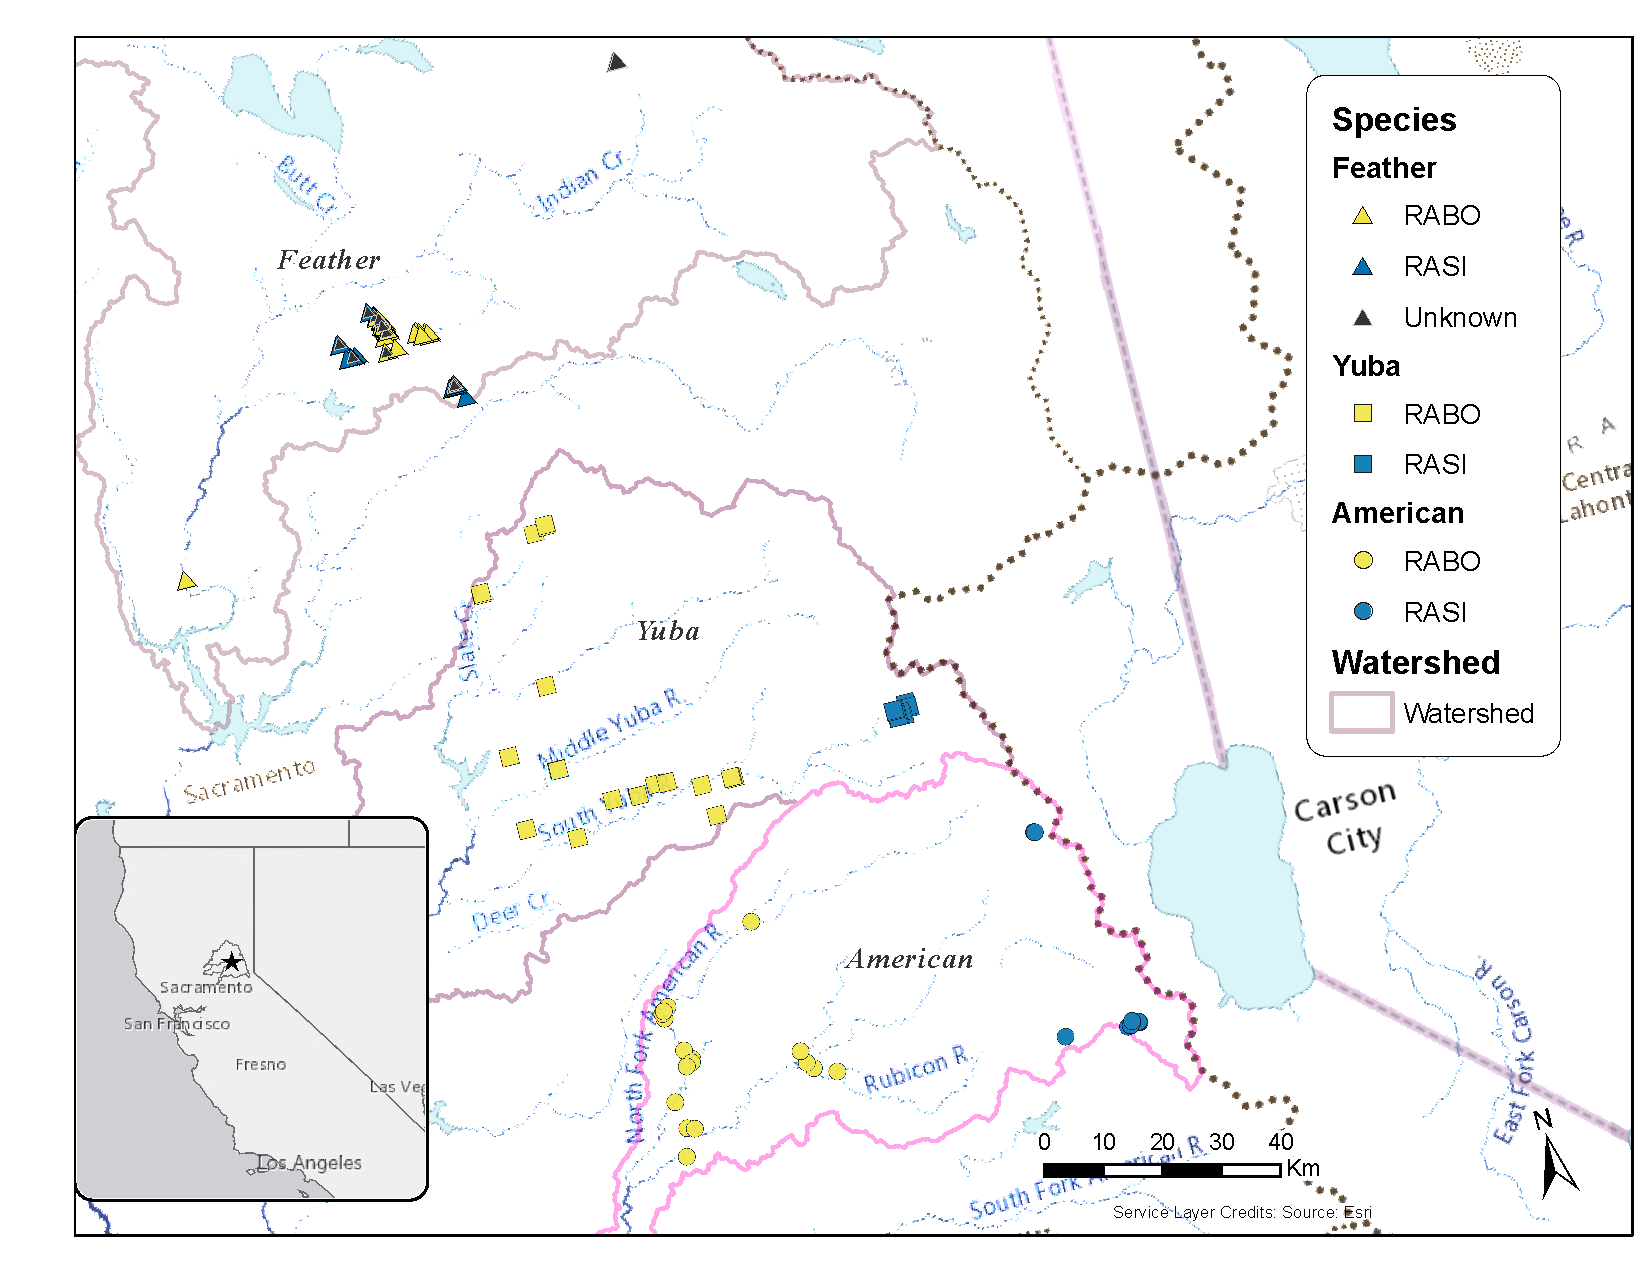
\includegraphics[angle=90, scale=.75]{figure/figure_01_overview_hybrid} \caption{Map of sampling locations in the Feather, Yuba, and
American watersheds. RABO=\emph{R. boylii}, RASI=\emph{R. sierrae}.}\label{fig:fig1map}
\end{figure}
\hypertarget{ref-labels}{%
\chapter{Tables, Graphics, References, and Labels}\label{ref-labels}}

\hypertarget{tables}{%
\section{Tables}\label{tables}}

By far the easiest way to present tables in your thesis is to store the
contents of the table in a CSV or Excel file, then read that file in to
your R Markdown document as a data frame. Then you can style the table
with the \texttt{kable} function, or functions in the
\href{https://cran.r-project.org/web/packages/kableExtra/index.html}{kableExtra}
pacakge.

In addition to the tables that can be automatically generated from a
data frame in \textbf{R} that you saw in {[}R Markdown Basics{]} using
the \texttt{kable} function, you can also create tables using
\emph{pandoc}. (More information is available at
\url{http://pandoc.org/README.html\#tables}.) This might be useful if
you don't have values specifically stored in \textbf{R}, but you'd like
to display them in table form. Below is an example. Pay careful
attention to the alignment in the table and hyphens to create the rows
and columns. Generally I don't recommend this approach of typing the
table directly into your R Markdown document.
\begin{longtable}[]{@{}ccc@{}}
\caption{\label{tab:inher} Correlation of Inheritance Factors for Parents
and Child}\tabularnewline
\toprule
\begin{minipage}[b]{0.29\columnwidth}\centering
Factors\strut
\end{minipage} & \begin{minipage}[b]{0.46\columnwidth}\centering
Correlation between Parents \& Child\strut
\end{minipage} & \begin{minipage}[b]{0.16\columnwidth}\centering
Inherited\strut
\end{minipage}\tabularnewline
\midrule
\endfirsthead
\toprule
\begin{minipage}[b]{0.29\columnwidth}\centering
Factors\strut
\end{minipage} & \begin{minipage}[b]{0.46\columnwidth}\centering
Correlation between Parents \& Child\strut
\end{minipage} & \begin{minipage}[b]{0.16\columnwidth}\centering
Inherited\strut
\end{minipage}\tabularnewline
\midrule
\endhead
\begin{minipage}[t]{0.29\columnwidth}\centering
Education\strut
\end{minipage} & \begin{minipage}[t]{0.46\columnwidth}\centering
-0.49\strut
\end{minipage} & \begin{minipage}[t]{0.16\columnwidth}\centering
Yes\strut
\end{minipage}\tabularnewline
\begin{minipage}[t]{0.29\columnwidth}\centering
Socio-Economic Status\strut
\end{minipage} & \begin{minipage}[t]{0.46\columnwidth}\centering
0.28\strut
\end{minipage} & \begin{minipage}[t]{0.16\columnwidth}\centering
Slight\strut
\end{minipage}\tabularnewline
\begin{minipage}[t]{0.29\columnwidth}\centering
Income\strut
\end{minipage} & \begin{minipage}[t]{0.46\columnwidth}\centering
0.08\strut
\end{minipage} & \begin{minipage}[t]{0.16\columnwidth}\centering
No\strut
\end{minipage}\tabularnewline
\begin{minipage}[t]{0.29\columnwidth}\centering
Family Size\strut
\end{minipage} & \begin{minipage}[t]{0.46\columnwidth}\centering
0.18\strut
\end{minipage} & \begin{minipage}[t]{0.16\columnwidth}\centering
Slight\strut
\end{minipage}\tabularnewline
\begin{minipage}[t]{0.29\columnwidth}\centering
Occupational Prestige\strut
\end{minipage} & \begin{minipage}[t]{0.46\columnwidth}\centering
0.21\strut
\end{minipage} & \begin{minipage}[t]{0.16\columnwidth}\centering
Slight\strut
\end{minipage}\tabularnewline
\bottomrule
\end{longtable}
We can also create a link to the table by doing the following: Table
\ref{tab:inher}. If you go back to {[}Loading and exploring data{]} and
look at the \texttt{kable} table, we can create a reference to this max
delays table too: Table \ref{tab:maxdelays}. The addition of the
\texttt{(\textbackslash{}\#tab:inher)} option to the end of the table
caption allows us to then make a reference to Table
\texttt{\textbackslash{}@ref(tab:label)}. Note that this reference could
appear anywhere throughout the document after the table has appeared.

\clearpage

\hypertarget{figures}{%
\section{Figures}\label{figures}}

If your thesis has a lot of figures, \emph{R Markdown} might behave
better for you than that other word processor. One perk is that it will
automatically number the figures accordingly in each chapter. You'll
also be able to create a label for each figure, add a caption, and then
reference the figure in a way similar to what we saw with tables
earlier. If you label your figures, you can move the figures around and
\emph{R Markdown} will automatically adjust the numbering for you. No
need for you to remember! So that you don't have to get too far into
LaTeX to do this, a couple \textbf{R} functions have been created for
you to assist. You'll see their use below.

In the \textbf{R} chunk below, we will load in a picture stored as
\texttt{uw.png} in our main directory. We then give it the caption of
``UW logo'', the label of ``uwlogo'', and specify that this is a figure.
Make note of the different \textbf{R} chunk options that are given in
the R Markdown file (not shown in the knitted document).
\begin{Shaded}
\begin{Highlighting}[]
\CommentTok{#include_graphics(path = "figure/uw.png")}
\end{Highlighting}
\end{Shaded}
Here is a reference to the UW logo: Figure \ref{fig:uwlogo}. Note the
use of the \texttt{fig:} code here. By naming the \textbf{R} chunk that
contains the figure, we can then reference that figure later as done in
the first sentence here. We can also specify the caption for the figure
via the R chunk option \texttt{fig.cap}.

\clearpage

Below we will investigate how to save the output of an \textbf{R} plot
and label it in a way similar to that done above. Recall the
\texttt{flights} dataset from Chapter \ref{rmd-basics}. (Note that we've
shown a different way to reference a section or chapter here.) We will
next explore a bar graph with the mean flight departure delays by
airline from Portland for 2014. Note also the use of the \texttt{scale}
parameter which is discussed on the next page.
\begin{Shaded}
\begin{Highlighting}[]
\NormalTok{flights }\OperatorTok\StringTok{ }\KeywordTok{group_by}\NormalTok{(carrier) }\OperatorTok
\StringTok{  }\KeywordTok{summarize}\NormalTok{(}\DataTypeTok{mean_dep_delay =} \KeywordTok{mean}\NormalTok{(dep_delay)) }\OperatorTok
\StringTok{  }\KeywordTok{ggplot}\NormalTok{(}\KeywordTok{aes}\NormalTok{(}\DataTypeTok{x =}\NormalTok{ carrier, }\DataTypeTok{y =}\NormalTok{ mean_dep_delay)) }\OperatorTok{+}
\StringTok{  }\KeywordTok{geom_bar}\NormalTok{(}\DataTypeTok{position =} \StringTok{"identity"}\NormalTok{, }\DataTypeTok{stat =} \StringTok{"identity"}\NormalTok{, }\DataTypeTok{fill =} \StringTok{"red"}\NormalTok{)}
\end{Highlighting}
\end{Shaded}
Here is a reference to this image: Figure \ref{fig:delaysboxplot}.

A table linking these carrier codes to airline names is available at
\url{https://github.com/ismayc/pnwflights14/blob/master/data/airlines.csv}.

\clearpage

Next, we will explore the use of the \texttt{out.extra} chunk option,
which can be used to shrink or expand an image loaded from a file by
specifying \texttt{"scale=\ "}. Here we use the mathematical graph
stored in the ``subdivision.pdf'' file.
\begin{figure}
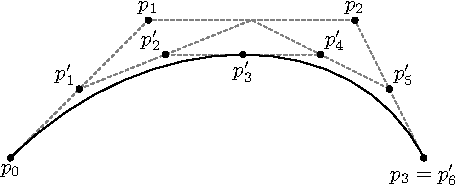
\includegraphics[scale=0.75]{figure/subdivision} \caption{Subdiv. graph}\label{fig:subd}
\end{figure}
Here is a reference to this image: Figure \ref{fig:subd}. Note that
\texttt{echo=FALSE} is specified so that the \textbf{R} code is hidden
in the document.

\textbf{More Figure Stuff}

Lastly, we will explore how to rotate and enlarge figures using the
\texttt{out.extra} chunk option. (Currently this only works in the PDF
version of the book.)
\begin{figure}
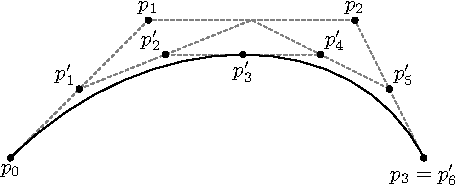
\includegraphics[angle=180, scale=1.1]{figure/subdivision} \caption{A Larger Figure, Flipped Upside Down}\label{fig:subd2}
\end{figure}
As another example, here is a reference: Figure \ref{fig:subd2}.

\hypertarget{footnotes-and-endnotes}{%
\section{Footnotes and Endnotes}\label{footnotes-and-endnotes}}

You might want to footnote something.\footnote{footnote text} The
footnote will be in a smaller font and placed appropriately. Endnotes
work in much the same way.

\hypertarget{bibliographies}{%
\section{Bibliographies}\label{bibliographies}}

Of course you will need to cite things, and you will probably accumulate
an armful of sources. There are a variety of tools available for
creating a bibliography database (stored with the .bib extension). In
addition to BibTeX suggested below, you may want to consider using the
free and easy-to-use tool called Zotero. Some Zotero documentation is at
\url{http://libguides.reed.edu/citation/zotero}. In addition, a tutorial
is available from Middlebury College at
\url{http://sites.middlebury.edu/zoteromiddlebury/}.

\emph{R Markdown} uses \emph{pandoc} (\url{http://pandoc.org/}) to build
its bibliographies. One nice caveat of this is that you won't have to do
a second compile to load in references as standard LaTeX requires. To
cite references in your thesis (after creating your bibliography
database), place the reference name inside square brackets and precede
it by the ``at'' symbol. For example, here's a reference to a book about
worrying: ({\textbf{???}}). This \texttt{Molina1994} entry appears in a
file called \texttt{thesis.bib} in the \texttt{bib} folder. This
bibliography database file was created by a program called BibTeX. You
can call this file something else if you like (look at the YAML header
in the main .Rmd file) and, by default, is to placed in the \texttt{bib}
folder.

For more information about BibTeX and bibliographies, see
(\url{http://web.reed.edu/cis/help/latex/index.html})\footnote{({\textbf{???}})}.
There are three pages on this topic: \emph{bibtex} (which talks about
using BibTeX, at \url{http://web.reed.edu/cis/help/latex/bibtex.html}),
\emph{bibtexstyles} (about how to find and use the bibliography style
that best suits your needs, at
\url{http://web.reed.edu/cis/help/latex/bibtexstyles.html}) and
\emph{bibman} (which covers how to make and maintain a bibliography by
hand, without BibTeX, at
\url{http://web.reed.edu/cis/help/latex/bibman.html}). The last page
will not be useful unless you have only a few sources.

If you look at the YAML header at the top of the main .Rmd file you can
see that we can specify the style of the bibliography by referencing the
appropriate csl file. You can download a variety of different style
files at \url{https://www.zotero.org/styles}. Make sure to download the
file into the csl folder.

\textbf{Tips for Bibliographies}
\begin{itemize}
\tightlist
\item
  Like with thesis formatting, the sooner you start compiling your
  bibliography for something as large as thesis, the better.
\item
  The cite key (a citation's label) needs to be unique from the other
  entries.
\item
  When you have more than one author or editor, you need to separate
  each author's name by the word ``and'' e.g.
  \texttt{Author\ =\ \{Noble,\ Sam\ and\ Youngberg,\ Jessica\},}.
\item
  Bibliographies made using BibTeX (whether manually or using a manager)
  accept LaTeX markup, so you can italicize and add symbols as
  necessary.
\item
  To force capitalization in an article title or where all lowercase is
  generally used, bracket the capital letter in curly braces.
\end{itemize}
\hypertarget{anything-else}{%
\section{Anything else?}\label{anything-else}}

If you'd like to see examples of other things in this template, please
\href{https://github.com/benmarwick/huskydown/issues/new}{contact us}
(email \href{mailto:bmarwick@uw.edu}{\nolinkurl{bmarwick@uw.edu}}) with
your suggestions. We love to see people using \emph{R Markdown} for
their theses, and are happy to help.

\appendix

\hypertarget{the-first-appendix}{%
\chapter{The First Appendix}\label{the-first-appendix}}

This first appendix includes all of the R chunks of code that were
hidden throughout the document (using the \texttt{include\ =\ FALSE}
chunk tag) to help with readibility and/or setup.

\textbf{In the main Rmd file}
\begin{Shaded}
\begin{Highlighting}[]
\CommentTok{# This chunk ensures that the huskydown package is}
\CommentTok{# installed and loaded. This huskydown package includes}
\CommentTok{# the template files for the thesis.}
\ControlFlowTok{if}\NormalTok{(}\OperatorTok{!}\KeywordTok{require}\NormalTok{(devtools))}
  \KeywordTok{install.packages}\NormalTok{(}\StringTok{"devtools"}\NormalTok{, }\DataTypeTok{repos =} \StringTok{"http://cran.rstudio.com"}\NormalTok{)}
\ControlFlowTok{if}\NormalTok{(}\OperatorTok{!}\KeywordTok{require}\NormalTok{(huskydown))}
\NormalTok{  devtools}\OperatorTok{::}\KeywordTok{install_github}\NormalTok{(}\StringTok{"benmarwick/huskydown"}\NormalTok{)}
\KeywordTok{library}\NormalTok{(huskydown)}
\CommentTok{#if(!require(huskydown))}
\CommentTok{#  devtools::install_github("danovando/gauchodown")}
\CommentTok{#library(gauchodown)}
\KeywordTok{library}\NormalTok{(knitr)}
\end{Highlighting}
\end{Shaded}
\textbf{In Chapter \ref{ref-labels}:}

\hypertarget{the-second-appendix-for-fun}{%
\chapter{The Second Appendix, for
Fun}\label{the-second-appendix-for-fun}}

\hypertarget{colophon}{%
\chapter*{Colophon}\label{colophon}}
\addcontentsline{toc}{chapter}{Colophon}

This document is set in \href{https://github.com/georgd/EB-Garamond}{EB
Garamond}, \href{https://github.com/adobe-fonts/source-code-pro/}{Source
Code Pro} and \href{http://www.latofonts.com/lato-free-fonts/}{Lato}.
The body text is set at 11pt with \(\familydefault\).

It was written in R Markdown and \(\LaTeX\), and rendered into PDF using
\href{https://github.com/benmarwick/huskydown}{huskydown} and
\href{https://github.com/rstudio/bookdown}{bookdown}.

This document was typeset using the XeTeX typesetting system, and the
\href{http://staff.washington.edu/fox/tex/}{University of Washington
Thesis class} class created by Jim Fox. Under the hood, the
\href{https://github.com/UWIT-IAM/UWThesis}{University of Washington
Thesis LaTeX template} is used to ensure that documents conform
precisely to submission standards. Other elements of the document
formatting source code have been taken from the
\href{https://github.com/stevenpollack/ucbthesis}{Latex, Knitr, and
RMarkdown templates for UC Berkeley's graduate thesis}, and
\href{https://github.com/suchow/Dissertate}{Dissertate: a LaTeX
dissertation template to support the production and typesetting of a PhD
dissertation at Harvard, Princeton, and NYU}

The source files for this thesis, along with all the data files, have
been organised into an R package, xxx, which is available at
\url{https://github.com/xxx/xxx}. A hard copy of the thesis can be found
in the University of Washington library.

This version of the thesis was generated on 2018-09-05 00:04:31. The
repository is currently at this commit:

The computational environment that was used to generate this version is
as follows:
\begin{verbatim}
Session info -------------------------------------------------------------
\end{verbatim}
\begin{verbatim}
 setting  value                       
 version  R version 3.5.1 (2018-07-02)
 system   x86_64, darwin15.6.0        
 ui       X11                         
 language (EN)                        
 collate  en_US.UTF-8                 
 tz       America/Los_Angeles         
 date     2018-09-05                  
\end{verbatim}
\begin{verbatim}
Packages -----------------------------------------------------------------
\end{verbatim}
\begin{verbatim}
 package     * version    date       source                               
 assertthat    0.2.0      2017-04-11 CRAN (R 3.5.0)                       
 backports     1.1.2      2017-12-13 CRAN (R 3.5.0)                       
 base        * 3.5.1      2018-07-05 local                                
 bindr         0.1.1      2018-03-13 CRAN (R 3.5.0)                       
 bindrcpp      0.2.2      2018-03-29 CRAN (R 3.5.0)                       
 bookdown    * 0.7        2018-02-18 CRAN (R 3.5.0)                       
 broom         0.5.0      2018-07-17 CRAN (R 3.5.0)                       
 cellranger    1.1.0      2016-07-27 CRAN (R 3.5.0)                       
 cli           1.0.0      2017-11-05 CRAN (R 3.5.0)                       
 colorspace    1.3-2      2016-12-14 CRAN (R 3.5.0)                       
 compiler      3.5.1      2018-07-05 local                                
 crayon        1.3.4      2017-09-16 CRAN (R 3.5.0)                       
 datasets    * 3.5.1      2018-07-05 local                                
 devtools    * 1.13.6     2018-06-27 CRAN (R 3.5.0)                       
 digest        0.6.16     2018-08-22 CRAN (R 3.5.1)                       
 dplyr       * 0.7.6      2018-06-29 CRAN (R 3.5.0)                       
 evaluate      0.11       2018-07-17 CRAN (R 3.5.0)                       
 forcats     * 0.3.0      2018-02-19 CRAN (R 3.5.0)                       
 ggplot2     * 3.0.0.9000 2018-09-04 Github (tidyverse/ggplot2@6e545dc)   
 git2r         0.23.0     2018-07-17 CRAN (R 3.5.0)                       
 glue          1.3.0      2018-07-17 CRAN (R 3.5.0)                       
 graphics    * 3.5.1      2018-07-05 local                                
 grDevices   * 3.5.1      2018-07-05 local                                
 grid          3.5.1      2018-07-05 local                                
 gtable        0.2.0      2016-02-26 CRAN (R 3.5.0)                       
 haven         1.1.2      2018-06-27 CRAN (R 3.5.0)                       
 hms           0.4.2      2018-03-10 CRAN (R 3.5.0)                       
 htmltools     0.3.6      2017-04-28 CRAN (R 3.5.0)                       
 httr          1.3.1      2017-08-20 CRAN (R 3.5.0)                       
 huskydown   * 0.0.5      2018-09-04 Github (benmarwick/huskydown@3ef00c9)
 jsonlite      1.5        2017-06-01 CRAN (R 3.5.0)                       
 kableExtra  * 0.9.0      2018-05-21 CRAN (R 3.5.0)                       
 knitr       * 1.20       2018-02-20 CRAN (R 3.5.0)                       
 lattice       0.20-35    2017-03-25 CRAN (R 3.5.1)                       
 lazyeval      0.2.1      2017-10-29 CRAN (R 3.5.0)                       
 lubridate     1.7.4      2018-04-11 CRAN (R 3.5.0)                       
 magrittr      1.5        2014-11-22 CRAN (R 3.5.0)                       
 memoise       1.1.0      2017-04-21 CRAN (R 3.5.0)                       
 methods     * 3.5.1      2018-07-05 local                                
 modelr        0.1.2      2018-05-11 CRAN (R 3.5.0)                       
 munsell       0.5.0      2018-06-12 CRAN (R 3.5.0)                       
 nlme          3.1-137    2018-04-07 CRAN (R 3.5.1)                       
 pillar        1.3.0      2018-07-14 CRAN (R 3.5.0)                       
 pkgconfig     2.0.2      2018-08-16 CRAN (R 3.5.0)                       
 plyr          1.8.4      2016-06-08 CRAN (R 3.5.0)                       
 purrr       * 0.2.5      2018-05-29 CRAN (R 3.5.0)                       
 R6            2.2.2      2017-06-17 CRAN (R 3.5.0)                       
 Rcpp          0.12.18    2018-07-23 CRAN (R 3.5.1)                       
 readr       * 1.1.1      2017-05-16 CRAN (R 3.5.0)                       
 readxl        1.1.0      2018-04-20 CRAN (R 3.5.0)                       
 rlang         0.2.2      2018-08-16 CRAN (R 3.5.0)                       
 rmarkdown     1.10       2018-06-11 cran (@1.10)                         
 rprojroot     1.3-2      2018-01-03 CRAN (R 3.5.0)                       
 rstudioapi    0.7        2017-09-07 CRAN (R 3.5.0)                       
 rvest         0.3.2      2016-06-17 CRAN (R 3.5.0)                       
 scales        1.0.0.9000 2018-08-29 Github (hadley/scales@0f7a186)       
 stats       * 3.5.1      2018-07-05 local                                
 stringi       1.2.4      2018-07-20 CRAN (R 3.5.0)                       
 stringr     * 1.3.1      2018-05-10 CRAN (R 3.5.0)                       
 tibble      * 1.4.2      2018-01-22 CRAN (R 3.5.0)                       
 tidyr       * 0.8.1      2018-05-18 CRAN (R 3.5.0)                       
 tidyselect    0.2.4      2018-02-26 CRAN (R 3.5.0)                       
 tidyverse   * 1.2.1      2017-11-14 CRAN (R 3.5.0)                       
 tools         3.5.1      2018-07-05 local                                
 utils       * 3.5.1      2018-07-05 local                                
 viridisLite   0.3.0      2018-02-01 CRAN (R 3.5.0)                       
 withr         2.1.2      2018-08-29 Github (jimhester/withr@8b9cee2)     
 xfun          0.3        2018-07-06 CRAN (R 3.5.0)                       
 xml2          1.2.0      2018-01-24 CRAN (R 3.5.0)                       
 yaml          2.2.0      2018-07-25 CRAN (R 3.5.0)                       
\end{verbatim}
\backmatter

\hypertarget{references}{%
\chapter*{References}\label{references}}
\addcontentsline{toc}{chapter}{References}

\markboth{References}{References}

\noindent

\setlength{\parindent}{-0.20in}
\setlength{\leftskip}{0.20in}
\setlength{\parskip}{8pt}

\hypertarget{refs}{}
\leavevmode\hypertarget{ref-abbott_hybridization_2013}{}%
Abbott, R., D. Albach, S. Ansell, J. W. Arntzen, S. J. E. Baird, N.
Bierne, J. Boughman, A. Brelsford, C. A. Buerkle, R. Buggs, R. K.
Butlin, U. Dieckmann, F. Eroukhmanoff, A. Grill, S. H. Cahan, J. S.
Hermansen, G. Hewitt, A. G. Hudson, C. Jiggins, J. Jones, B. Keller, T.
Marczewski, J. Mallet, P. Martinez-Rodriguez, M. Möst, S. Mullen, R.
Nichols, A. W. Nolte, C. Parisod, K. Pfennig, A. M. Rice, M. G. Ritchie,
B. Seifert, C. M. Smadja, R. Stelkens, J. M. Szymura, R. Väinölä, J. B.
W. Wolf, and D. Zinner. 2013. Hybridization and speciation. Journal of
evolutionary biology 26:229--246.

\leavevmode\hypertarget{ref-ali_rad_2016}{}%
Ali, O. A., S. M. O'Rourke, S. J. Amish, M. H. Meek, G. Luikart, C.
Jeffres, and M. R. Miller. 2016. RAD Capture (Rapture): Flexible and
Efficient Sequence-Based Genotyping. Genetics 202:389--400.

\leavevmode\hypertarget{ref-baird_descriptions_1856}{}%
Baird, S. F. 1856. Descriptions of new genera and species of North
American Frogs. Pages 59--62 \emph{in} Proceedings of the Academy of
Natural Sciences of Philadelphia. Philadelphia, Academy of Natural
Sciences of Philadelphia.

\leavevmode\hypertarget{ref-barrera-guzman_hybrid_2018}{}%
Barrera-Guzmán, A. O., A. Aleixo, M. D. Shawkey, and J. T. Weir. 2018.
Hybrid speciation leads to novel male secondary sexual ornamentation of
an Amazonian bird. Proceedings of the National Academy of Sciences of
the United States of America 115:E218--E225.

\leavevmode\hypertarget{ref-bunn_basic_2002}{}%
Bunn, S. E., and A. H. Arthington. 2002. Basic principles and ecological
consequences of altered flow regimes for aquatic biodiversity.
Environmental management 30:492--507.

\leavevmode\hypertarget{ref-camp_notes_1917}{}%
Camp, C. L. 1917. Notes on the systematic status of the toads and frogs
of California. University of California publications in zoology
17:115--125.

\leavevmode\hypertarget{ref-caze_could_2016}{}%
Cazé, A. L. R., G. Mäder, T. S. Nunes, L. P. Queiroz, G. de Oliveira, J.
A. F. Diniz-Filho, S. L. Bonatto, and L. B. Freitas. 2016. Could refuge
theory and rivers acting as barriers explain the genetic variability
distribution in the Atlantic Forest? Molecular phylogenetics and
evolution 101:242--251.

\leavevmode\hypertarget{ref-drost_collapse_1996}{}%
Drost, C. A., and G. M. Fellers. 1996. Collapse of a Regional Frog Fauna
in the Yosemite Area of the California Sierra Nevada, USA. Conservation
biology: the journal of the Society for Conservation Biology
10:414--425.

\leavevmode\hypertarget{ref-dudgeon_freshwater_2006}{}%
Dudgeon, D., A. H. Arthington, M. O. Gessner, Z.-I. Kawabata, D. J.
Knowler, C. Lévêque, R. J. Naiman, A.-H. Prieur-Richard, D. Soto, M. L.
J. Stiassny, and C. A. Sullivan. 2006. Freshwater biodiversity:
Importance, threats, status and conservation challenges. Biological
reviews of the Cambridge Philosophical Society 81:163--182.

\leavevmode\hypertarget{ref-li_ten_2017}{}%
Li, Y., X.-X. Zhang, R.-L. Mao, J. Yang, C.-Y. Miao, Z. Li, and Y.-X.
Qiu. 2017. Ten Years of Landscape Genomics: Challenges and
Opportunities. Frontiers in plant science 8:2136.

\leavevmode\hypertarget{ref-mallet_hybrid_2007}{}%
Mallet, J. 2007. Hybrid speciation. Nature 446:279--283.

\leavevmode\hypertarget{ref-moyle_rapid_2011}{}%
Moyle, P. B., J. V. E. Katz, and R. M. Quiñones. 2011. Rapid decline of
California's native inland fishes: A status assessment. Biological
conservation 144:2414--2423.

\leavevmode\hypertarget{ref-murchie_fish_2008}{}%
Murchie, K. J., K. P. E. Hair, C. E. Pullen, T. D. Redpath, H. R.
Stephens, and S. J. Cooke. 2008. Fish response to modified flow regimes
in regulated rivers: Research methods, effects and opportunities. River
research and applications 24:197--217.

\leavevmode\hypertarget{ref-nilsson_fragmentation_2005}{}%
Nilsson, C., C. A. Reidy, M. Dynesius, and C. Revenga. 2005.
Fragmentation and flow regulation of the world's large river systems.
Science 308:405--408.

\leavevmode\hypertarget{ref-poff_homogenization_2007}{}%
Poff, N. L., J. D. Olden, D. M. Merritt, and D. M. Pepin. 2007.
Homogenization of regional river dynamics by dams and global
biodiversity implications. Proceedings of the National Academy of
Sciences of the United States of America 104:5732--5737.

\leavevmode\hypertarget{ref-power_dams_1996}{}%
Power, M. E., W. E. Dietrich, and J. C. Finlay. 1996. Dams and
Downstream Aquatic Biodiversity: Potential Food Web Consequences of
Hydrologic and Geomorphic Change. Environmental management 20:887--895.

\leavevmode\hypertarget{ref-prince_evolutionary_2017}{}%
Prince, D. J., S. M. O'Rourke, T. Q. Thompson, O. A. Ali, H. S. Lyman,
I. K. Saglam, T. J. Hotaling, A. P. Spidle, and M. R. Miller. 2017. The
evolutionary basis of premature migration in Pacific salmon highlights
the utility of genomics for informing conservation. Science advances
3:e1603198.

\leavevmode\hypertarget{ref-pringle_what_2003}{}%
Pringle, C. 2003. What is hydrologic connectivity and why is it
ecologically important? Hydrological processes 17:2685--2689.

\leavevmode\hypertarget{ref-pringle_hydrologic_2001}{}%
Pringle, C. M. 2001. Hydrologic Connectivity and the Management of
Biological Reserves: A Global Perspective. Ecological applications: a
publication of the Ecological Society of America 11:981--998.

\leavevmode\hypertarget{ref-schick_directed_2007}{}%
Schick, R. S., and S. T. Lindley. 2007. Directed connectivity among fish
populations in a riverine network. The Journal of applied ecology
44:1116--1126.

\leavevmode\hypertarget{ref-shaffer_species_2004}{}%
Shaffer, H. B., G. M. Fellers, S. R. Voss, J. C. Oliver, and G. B.
Pauly. 2004. Species boundaries, phylogeography and conservation
genetics of the red-legged frog (Rana aurora/draytonii) complex.
Molecular ecology 13:2667--2677.

\leavevmode\hypertarget{ref-shaw_importance_2016}{}%
Shaw, E. A., E. Lange, J. D. Shucksmith, and D. N. Lerner. 2016.
Importance of partial barriers and temporal variation in flow when
modelling connectivity in fragmented river systems. Ecological
engineering 91:515--528.

\leavevmode\hypertarget{ref-stebbins_field_2003}{}%
Stebbins, R. C. 2003. A Field Guide to Western Reptiles and Amphibians.
3rd editions. Houghton Mifflin Harcourt, Boston.

\leavevmode\hypertarget{ref-tonkin_seasonality_2017}{}%
Tonkin, J. D., M. T. Bogan, N. Bonada, B. Rios-Touma, and D. A. Lytle.
2017. Seasonality and predictability shape temporal species diversity.
Ecology 98:1201--1216.

\leavevmode\hypertarget{ref-usfws_endangered_2014}{}%
USFWS. 2014. Endangered and Threatened Wildlife and Plants; Endangered
Species Status for Sierra Nevada Yellow-Legged Frog and Northern
Distinct Population Segment of the Mountain Yellow-Legged Frog, and
Threatened Species Status for Yosemite Toad. Federal register
79:24255--24310.

\leavevmode\hypertarget{ref-voelker_river_2013}{}%
Voelker, G., B. D. Marks, C. Kahindo, U. A'genonga, F. Bapeamoni, L. E.
Duffie, J. W. Huntley, E. Mulotwa, S. A. Rosenbaum, and J. E. Light.
2013. River barriers and cryptic biodiversity in an evolutionary museum.
Ecology and evolution 3:536--545.

\leavevmode\hypertarget{ref-wiens_riverine_2002}{}%
Wiens, J. A. 2002. Riverine landscapes: Taking landscape ecology into
the water. Freshwater biology 47:501--515.

\leavevmode\hypertarget{ref-yarnell_ecology_2010}{}%
Yarnell, S. M., J. H. Viers, and J. F. Mount. 2010. Ecology and
Management of the Spring Snowmelt Recession. Bioscience 60:114--127.

\leavevmode\hypertarget{ref-zweifel_ecology_1955}{}%
Zweifel, R. G. 1955. Ecology, distribution, and systematics of frogs of
the Rana boylei group. University of California publications in zoology
54:207--291.

\end{ucmainmatter}
\end{document}

%---Set Headers and Footers ------------------------------------------------------
\pagestyle{fancy}
\renewcommand{\chaptermark}[1]{\markboth{{\sf #1 \hspace*{\fill} Chapter~}}{} }
\renewcommand{\sectionmark}[1]{\markright{ {\sf Section~\thesection \hspace*{\fill} #1 }}}
\fancyhf{}

\makeatletter \if@twoside \fancyhead[LO]{\small \rightmark} \fancyhead[RE]{\small\leftmark} \else \fancyhead[LO]{\small\leftmark}
\fancyhead[RE]{\small\rightmark} \fi

\def\cleardoublepage{\clearpage\if@openright \ifodd\c@page\else
  \hbox{}
  \vspace*{\fill}
  \begin{center}
    This page intentionally left blank
  \end{center}
  \vspace{\fill}
  \thispagestyle{plain}
  \newpage
  \fi \fi}
\makeatother
\fancyfoot[c]{\textrm{\textup{\thepage}}} % page number
\fancyfoot[C]{\thepage}
\setlength\footskip{-2pt}
\renewcommand{\headrulewidth}{0.4pt}

\fancypagestyle{plain} { \fancyhf{} \fancyfoot[C]{\thepage}
\renewcommand{\headrulewidth}{0pt}
\renewcommand{\footrulewidth}{0pt}}
